\documentclass[11pt,a4paper]{article}
% \usepackage[T1]{fontenc}\usepackage{lmodern}  % optional, if Latin Modern is installed
\usepackage[utf8]{inputenc}
\usepackage[margin=2.3cm]{geometry}
\usepackage{amsmath,amssymb}
\usepackage{booktabs,array}
\usepackage{authblk}
\usepackage{xcolor}
\usepackage{textcomp}
\usepackage{upquote}
\usepackage{listings}
\usepackage{pgfplots}
\pgfplotsset{compat=1.15}
\usepackage[colorlinks=true,linkcolor=blue!50!black,citecolor=blue!50!black,urlcolor=blue!50!black]{hyperref}

\definecolor{codebg}{gray}{0.965}
\definecolor{codegreen}{rgb}{0.10,0.45,0.10}
\definecolor{codeblue}{rgb}{0.05,0.20,0.55}
\lstset{language=Python,basicstyle=\ttfamily\scriptsize,columns=fullflexible,keepspaces=true,
  upquote=true,showstringspaces=false,breaklines=true,breakatwhitespace=false,
  postbreak=\mbox{\textcolor{gray}{$\hookrightarrow$}\space},
  backgroundcolor=\color{codebg},frame=single,rulecolor=\color{gray!40},
  commentstyle=\color{codegreen},keywordstyle=\color{codeblue},stringstyle=\color{red!45!black},
  numbers=left,numberstyle=\tiny\color{gray},numbersep=6pt,xleftmargin=1.4em,
  literate={~}{{\textasciitilde}}1}

\newcommand{\ainv}{\alpha^{-1}}
\newcommand{\kY}{k_Y}
\newcommand{\GeV}{\,\mathrm{GeV}}
\newcommand{\TeV}{\,\mathrm{TeV}}
\newcommand{\MU}{M_U}
\newcommand{\MPl}{M_{\mathrm{Pl}}}

\title{\textbf{Investigation by AI about the mysterious 137}\\[4pt]
\large A three-hour, human-steered dialogue between AI systems on the origin of the fine-structure constant}

\author[1]{Fable5.1}
\author[2]{GPT5.6-Sol}
\author[3]{l0d0v1c}
\author[3]{pseudoLuc}
\affil[1]{AI system (Claude Fable~5.1, Anthropic): calculations, scripts, literature checks, drafting}
\affil[2]{AI system: critical review and extension of the first half of the investigation}
\affil[3]{Questions, steering, relay between the AI systems, time-keeping}
% TODO (human authors): please check the three role descriptions above and amend them if needed.
\date{21 September 2026}

\begin{document}
\maketitle

\begin{abstract}
\noindent We report an experiment rather than a discovery. In about three hours of conversation, steered by
open questions and with one round of cross-criticism between two AI systems, an AI assistant equipped with a
Python sandbox and a web-search tool was asked whether the fine-structure constant $\alpha\simeq1/137.036$ might have
a geometric origin. The purpose was to see how far such a dialogue can go, and in particular whether it can
\emph{re-derive known results, possibly by other means}, while keeping track of its own errors.
The investigation (i) tested $4.8\times10^{6}$ products of volumes of symmetric spaces against four constants with a
decoy-target control, finding nothing beyond chance and recovering Wyler's 1969 formula as the unique hit of its class;
(ii) showed that Wyler's value lies \emph{above} the infrared floor of $\ainv$ and therefore cannot be $\alpha$ at any scale;
(iii) quantified the ``induced electrodynamics'' hypothesis and scanned $151{,}263$ vector-like spectra, rediscovering
the ``strong unification'' scenario and formulating a \emph{conservation lemma}: a rigid ultraviolet condition trades a
modulus for a threshold and removes no continuous parameter;
(iv) re-derived at two loops, from independent inputs, that the Standard Model alone unifies for a hypercharge
normalisation $\kY=1.341\pm0.004$, compatible with $\kY=4/3$, which then predicts $\ainv(0)=136.7$ ($-0.26\%$);
(v) connected $\kY=4/3$ to a point of enhanced symmetry in $SU(6)$ and, through a generalised Schellekens condition,
to fractional electric charges in units of $1/6$;
(vi) stress-tested that conclusion with Kaluza--Klein thresholds, Bayesian evidence, an intermediate supersymmetry
scale and the Higgs quartic coupling. Almost every positive result turned out to be already in the literature; we list
what was recovered, by which route, what was corrected along the way, and what such a dialogue cannot do.
All Python sources are reproduced in the appendix.
\end{abstract}

\tableofcontents

%======================================================================
\section{Introduction: the experiment}
%======================================================================

The number $1/137$ has a long record of attracting numerology \cite{Eddington,Wyler,Robertson}. It is therefore a good
stress test for an AI system: the topic rewards fluent speculation, punishes it quickly when numbers are computed, and has
a large literature against which any claim can be checked.

\paragraph{Protocol.} The investigation was a single conversation of about three hours (wall-clock time, as kept by the
human participants). It started from a naive question, \emph{does $\alpha$ tend to an asymptote at high energy?}, and
proceeded by short prompts (``could it come from a geometry?'', ``can you try?'', ``do you have an idea?'', ``go on'').
The first AI system (Fable5.1) had access to a sandboxed Linux machine (Python~3 with \texttt{numpy} only) and to web
search. Midway, the working notes were submitted to a second AI system (GPT5.6-Sol), whose twelve-section critique was
pasted back into the conversation; the first system checked every number in it, conceded the points on which it was
wrong, objected where it disagreed, and continued. No human supplied physics content; the human role was to ask, to
choose which suggested follow-up to pursue, and at one point to ask whether it was worth continuing.

\paragraph{Aims.} (a) Recover established results, where possible by a route different from the original one.
(b) Attach to every numerical coincidence an estimate of how often chance does as well.
(c) Keep an explicit log of mistakes and retractions. (d) State clearly what remains unverified.

\paragraph{What this paper is not.} It is not a claim of new physics, and it has not been reviewed by a specialist.
The calculations are one- or two-loop estimates with unknown high-scale thresholds. Section~\ref{sec:limits} lists
the known weaknesses, including formulae recalled from the model's memory.

%======================================================================
\section{Background: what kind of number is \texorpdfstring{$\alpha$}{alpha}?}
%======================================================================

At one loop, for $Q\gg m_f$,
\begin{equation}
\alpha(Q^2)=\frac{\alpha_0}{1-\dfrac{\alpha_0}{3\pi}\sum_f Q_f^2N_c\ln\dfrac{Q^2}{m_f^2}}\,,
\end{equation}
so that $\ainv$ decreases logarithmically with energy, from $137.036$ at $Q=0$ to $\simeq127.95$ at $M_Z$, and formally
reaches a Landau pole far above the Planck scale. There is no high-energy asymptote. Below the electron mass, however,
nothing runs any more: $\ainv(0)=137.035999177$ \cite{CODATA} is an infrared \emph{floor}, the only true asymptote of the
curve. Above the electroweak scale the relevant quantities are the hypercharge and $SU(2)$ couplings, with
$\ainv_{\rm em}=\ainv_Y+\ainv_2$.

Two clarifications, both of which emerged from the cross-criticism step, frame everything that follows.
First, in the renormalised Standard Model $\alpha(0)$ is an \emph{input}. Fermion masses do not determine it; they only
relate the coupling at two scales. Masses become decisive only once an ultraviolet condition
$\ainv(\Lambda)=C$ is imposed, in which case $\ainv(0)=C+\text{running}+\text{thresholds}$.
Second, the identity $\alpha=Z_0/2R_K$, with $R_K=h/e^2$ the von Klitzing resistance, is a tautology: the topological
nature of the quantum Hall effect fixes the integer $\nu$ in $R_H=R_K/\nu$, not the ratio $R_K/Z_0$.

%======================================================================
\section{The direct geometric route, and why it fails}
%======================================================================

\subsection{What topology fixes and what it does not}
For a $U(1)$ gauge field,
\begin{equation}
S[A]=\frac{1}{2e^2}\int F\wedge{*F}+\frac{i\theta}{8\pi^2}\int F\wedge F .
\end{equation}
Fluxes $\frac{1}{2\pi}\int_\Sigma F$ are integers and $\theta$ is periodic, but the Maxwell term contains the Hodge star,
hence the metric, and its coefficient $1/e^2$ is continuous. A Chern number explains why charges are integers, not why two
unit charges interact with strength $1/137$. A rigid value requires something more: a symmetry (e.g.\ a fixed point of
an $SL(2,\mathbb Z)$ duality acting on $\tau=\theta/2\pi+i/\alpha$, which gives $\alpha\sim1$), a dynamical stabilisation,
a renormalisation-group fixed point, or a compositeness condition $1/e^2(\Lambda)=0$.

\subsection{Wyler's formula}
Wyler \cite{Wyler} proposed
\begin{equation}
\alpha_W=\frac{9}{8\pi^4}\left(\frac{\pi^5}{2^4\,5!}\right)^{1/4},\qquad \ainv_W=137.03608,
\end{equation}
from Hua's volumes \cite{Hua} of the type-IV Cartan domain $D^5=SO(5,2)/[SO(5)\times SO(2)]$, its Shilov boundary $Q^5$ and
$S^4$. The classical objections (no Lagrangian, arbitrary choice of $SO(5,2)$ and of the power $1/4$, normalisation-dependent
volumes) are due to Robertson \cite{Robertson} and others. The cross-criticism step supplied a sharper one:
\begin{quote}
$\ainv_W=137.03608$ is \emph{larger} than $\ainv(0)=137.035999$. Since screening implies $\ainv(Q^2)<\ainv(0)$ for all
$Q^2>0$, Wyler's number is on the wrong side of the infrared floor and cannot be reinterpreted as $\alpha$ at any scale.
\end{quote}

\subsection{Numerical tests with a look-elsewhere control}
\paragraph{Wyler's recipe in dimension $n$} (script~01) gives, for $n=3,\dots,8$, the values $\ainv=38.8$, $76.9$, $\mathbf{137.036}$, $225.7$, $349.8$, $515.9$: only $n=5$ lands near a physical value, and neither $128$ nor the unification values $25$--$47$ appear.

\paragraph{Wyler's class.} Among all numbers $2^a3^b5^c\pi^d$ with quarter-integer exponents in $[-6,6]$
($5.8\times10^6$ combinations), exactly one lies within $10^{-6}$ of $\ainv(0)$: Wyler's formula, recovered without being
put in. None lies within $10^{-7}$. The expected number of chance hits at $10^{-6}$ is $0.1$--$0.3$, so the usual
remark that ``one can get 137 from anything'' is too strong within this class, while the formula is nonetheless excluded
at today's precision.

\paragraph{Four Cartan families} (script~02). With 36 building blocks (Hua volumes of domains of types I--IV up to complex
dimension 10, spheres $S^1$--$S^8$, Shilov boundaries $Q^2$--$Q^8$), products of up to three blocks with exponents
$\pm\frac14,\pm\frac12,\pm1,\pm2$ and a small rational prefactor give $4.78\times10^6$ distinct values. For each target,
4000 decoy targets drawn within $\pm20\%$ estimate the chance rate (Table~\ref{tab:cartan}).

\begin{table}[h]\centering
\caption{Hits of the Cartan-volume family (script 02). ``Expected'' is the mean over 4000 local decoys.}\label{tab:cartan}
\begin{tabular}{lccc}\toprule
Target & hits at $10^{-5}$ (expected) & hits at $10^{-6}$ (expected) & hits at $10^{-7}$\\\midrule
$\ainv$ & 5 (4.1) & 2 (0.42) & 0\\
$m_\mu/m_e$ & 4 (3.9) & 1 (0.38) & 0\\
$m_p/m_e$ & 3 (3.0) & 0 (0.30) & 0\\
$m_n/m_e$ & 3 (3.0) & 0 (0.31) & 0\\\bottomrule
\end{tabular}\end{table}

The two hits for $\ainv$ are Wyler's formula and a meaningless mixture of a type-I domain, a type-III domain and $Q^4$ that
does slightly better ($4.4\times10^{-7}$): once the family is enlarged, Wyler loses uniqueness. The muon hit shares no block
with those of $\alpha$; $6\pi^5$ for $m_p/m_e$ stays at $2\times10^{-5}$, within the noise. \emph{The real constants behave
like generic numbers with respect to this family.}

%======================================================================
\section{The indirect route: ultraviolet condition, spectrum, running}
%======================================================================

If geometry matters, it must act indirectly: it fixes an ultraviolet condition, a spectrum and thresholds, and the
renormalisation group produces $\alpha(0)$.

\subsection{Induced electrodynamics and the spectral budget}
Following Landau and Zeldovich \cite{Landau,Zeldovich}, suppose the photon has no kinetic term of its own at a fundamental
scale: $\ainv_Y(\Lambda)=0$. With $\Lambda=\MPl=1.22\times10^{19}\GeV$, $b_Y^{\rm SM}=41/6$ and $\ln(\MPl/M_Z)=39.44$, the
Standard Model induces $\ainv_Y(M_Z)=42.9$ against a measured $98.4$; adding the measured $\ainv_2(M_Z)=29.6$ and the
$9.1$ units gained between $M_Z$ and $Q=0$ gives $\ainv(0)\simeq82$. The right order of magnitude with no free parameter,
but wrong by a factor $1.7$. The deficit is a \emph{spectral budget},
\begin{equation}\label{eq:budget}
\sum_j\Delta b_{Y,j}\ln\frac{\Lambda}{M_j}\simeq2\pi\times55.5\simeq348.7 ,
\end{equation}
which vector-like matter can fill: seven $Y{=}1$ Dirac leptons at $0.7\TeV$, two $Y{=}2$ fermions at $8\times10^4\GeV$, or
one $Y{=}3$ fermion at $3\times10^6\GeV$. These toy solutions (second AI system, checked by the first) show that the
pole condition is one \emph{integrated} constraint satisfied by infinitely many spectra. The first system added that
$\Lambda$ is itself a hidden continuous parameter, $M\propto\Lambda^{1+b_{\rm SM}/\Delta b}$: with the reduced Planck mass the
seven leptons drop from $726\GeV$ to about $45\GeV$, excluded since LEP. It also noted that an $SL(2,\mathbb Z)$
fixed point ($\ainv(\Lambda)\simeq1$) and induced electrodynamics ($\ainv(\Lambda)=0$) differ by $1\%$ of the budget and should
be treated as one family, ``rigid strong coupling at $\Lambda$'', $\ainv_i(\Lambda)\in[0,1]$, whose intrinsic precision
is about $1\%$.

\subsection{Scan of 151{,}263 spectra (script 03)}
We asked which matter contents make all three couplings strong at a common $\Lambda$. The family comprises the vector-like
representations contained in the $\mathbf5$, $\mathbf{10}$ and $\mathbf{24}$ of $SU(5)$, namely $E\,(1,1)_1$, $L\,(1,2)_{1/2}$,
$D\,(3,1)_{1/3}$, $U\,(3,1)_{2/3}$, $Q\,(3,2)_{1/6}$ with multiplicities $0$--$6$, and a real triplet and octet with
multiplicities $0$--$2$, all at a common mass $M\ge1\TeV$, on a Standard Model base or an MSSM base with superpartners
at $M$. As a control, the three measured couplings were replaced by ``decoy worlds'' drawn within a factor $1.25$--$2$.

\begin{table}[h]\centering
\caption{Spectra for which $(\Lambda,M)$ exist with $0\le\ainv_i(\Lambda)\le1$ for $i=Y,2,3$ (scripts 03 and 08). Decoy medians are for a spread factor $1.5$ unless stated.}\label{tab:scan}
\small\begin{tabular}{llccc}\toprule
Base & $\Lambda$ & compatible & decoy median & $P(\text{decoy}\ge\text{real})$\\\midrule
SM, one mass & free ($10^{10}$--$10^{19}$ GeV) & 2565 (1.7\%) & 1743 & 0.39--0.49\\
SM, one mass & Planck window & 645 (0.43\%) & 242 & 0.013--0.05\\
MSSM, one mass & Planck window & 1110 (0.73\%) & 688 ($\times1.25$) & 0.025\\
SM, two masses & free & 12{,}912 (8.5\%) & -- & --\\
SM, two masses & Planck window & 4941 (3.3\%) & 2438 & 0.06--0.31\\\bottomrule
\end{tabular}\end{table}

With $\Lambda$ free the condition has no explanatory power: thousands of spectra qualify and our world is typical.
With $\Lambda$ in the window $[2.4\times10^{18},1.22\times10^{19}]\GeV$ our world looked mildly favoured ($p\simeq1$--$5\%$).
The cause was identified: at that scale the required $\Delta b_i$ are nearly equal, $(8.84,7.88,8.35)$, which generic matter
provides easily; a fictitious world requiring exactly equal $\Delta b_i$ obtains 639 spectra against 641 for ours, while
unbalanced requirements give $266$, $44$, $8$, $0$. The preference did not survive a second mass scale
(coloured and uncoloured multiplets at different masses, script~08): $p$ rose to $0.06$--$0.31$. We file it as a fluctuation.

\paragraph{A rediscovery.} On the MSSM base the only complete-$SU(5)$-multiplet solutions are
$(n_5,n_{10})=(6,0),(3,1),(4,1),(0,2),(1,2)$, i.e.\ $n_5+3n_{10}=6$ or $7$, with $\Lambda\simeq10^{16}\GeV$ and
$M\simeq8$--$80\TeV$: the brute-force scan lands, unprompted, on the ``strong unification''/``universal Landau pole''
scenario \cite{MPP,GLR,ULP}. On the Standard Model base no complete multiplet works, as the first system had argued beforehand:
equal $\Delta b_i$ in $SU(5)$ normalisation leave coupling differences intact, so a common pole would require the Standard
Model to unify already with $\kY=5/3$, which it does not.

\subsection{A conservation lemma}
In the best structured case (MSSM plus $n=n_5+3n_{10}$ multiplets, common strong coupling, $\Lambda$ fitted to $\alpha_s$),
$\ainv(0)$ is predicted (script~04): $n=6$ gives $126.6$--$119.9$ for $M=3\TeV$, $\mathbf{139.8}$--$\mathbf{133.1}$ for
$M=10\TeV$ and $151.8$--$145.2$ for $M=30\TeV$ (the range corresponds to $\ainv_i(\Lambda)\in[0,1]$). One can get $137$, but
\begin{equation}
\frac{d\,\ainv(0)}{d\ln M}\simeq11 .
\end{equation}
\begin{quote}\textbf{Lemma (conservation of the free parameter).} A rigid ultraviolet condition does not reduce the number of
continuous parameters. Ordinary grand unification has $(\MU,\alpha_U)$; rigid strong coupling has $(\Lambda,M)$. In both cases
there are three observables, two parameters and one prediction. The modulus $\alpha_U$ is exchanged for the threshold $M$, at
a rate of $8/3$ per unit of $\ainv_U$ against $11$ per $e$-fold of $M$.\end{quote}
Every specialist knows this implicitly; we have not seen it phrased this way, and it recurs below in a second guise
(Section~\ref{sec:degeneracy}).

\paragraph{The only escape.} A prediction requires $\ln(\Lambda/M)$ itself to be discrete. Dimensional transmutation of a
hidden gauge sector gives $M=\Lambda\exp[-2\pi\ainv_h(\Lambda)/b_h]$. A rigid \emph{strong} coupling cannot generate a large
hierarchy (for a confining sector $b_h\gtrsim5$ gives $\ln(\Lambda/M)\lesssim1$, and small $b_h$ leads into the conformal
window), so the hidden coupling must be \emph{weak}, $\ainv_h(\Lambda)=N_h\gg1$. If $N_h$ is discrete (a flux, a rank), then at
leading order $\ainv_i(M_Z)=N_i+b_iN_{\rm EW}/b_{\rm EW}+\Delta b_iN_h/b_h$ is an explicit function of integers. Two-loop and
threshold corrections amount to a few units, so these integers \emph{cannot} be read off $137.036$; we deliberately did not scan
for them, since the theoretical error exceeds the spacing of candidates.

%======================================================================
\section{Where discreteness really enters: the hypercharge normalisation}
%======================================================================

\subsection{A two-loop re-derivation}
One discrete, geometric datum does touch $\alpha$: the normalisation $\kY$ in $\alpha_1=\kY\alpha_Y$. In heterotic string
theory $k_i\,\ainv_{\rm string}=\ainv_i$ with $k_i$ the levels of the world-sheet current algebras \cite{DienesReview}; this
realises the idea ``level of a current algebra $\to$ coupling'', but fixes only \emph{ratios}. The canonical $SU(5)$ value is $5/3$.

We took as inputs the $\overline{\rm MS}$ couplings at $\mu=M_t$ extracted at NNLO by Buttazzo et al.\ \cite{Buttazzo},
$\ainv_Y=97.885$, $\ainv_2=29.946$, $\ainv_3=9.262$ (for $\alpha_s(M_Z)=0.1180$), and ran the two-loop Standard Model
equations \cite{MV} with the top Yukawa (script~05). Defining $\MU$ by $\alpha_2=\alpha_3$:
\begin{center}\begin{tabular}{lccc}\toprule
 & $\MU$ & $\ainv_U$ & required $\kY$\\\midrule
one loop & $9.2\times10^{16}\GeV$ & 47.03 & 1.297\\
two loops & $2.9\times10^{16}\GeV$ & 46.18 & $\mathbf{1.341\pm0.004}$\\\bottomrule
\end{tabular}\end{center}
The error reflects $\alpha_s(M_Z)=0.1180\pm0.0009$; the top-mass uncertainty is negligible. Fitting $(\MU,\alpha_U)$ to
$\alpha_2,\alpha_3$ and \emph{predicting} $\alpha_Y$, hence $\ainv(0)$, gives Table~\ref{tab:kY}.

\begin{table}[h]\centering
\caption{Predicted $\ainv(0)$ for rational $\kY$, Standard Model only (script 05). Measured: $137.036$.}\label{tab:kY}
\begin{tabular}{lccccccc}\toprule
$\kY$ & $5/3$ & $\mathbf{4/3}$ & $13/10$ & $32/25$ & $5/4$ & $6/5$ & $1$\\\midrule
one loop & 154.4 & 138.7 & 137.2 & 136.2 & 134.8 & 132.5 & 123.1\\
two loops & 152.1 & \textbf{136.68} & 135.1 & 134.2 & 132.8 & 130.5 & 121.3\\
deviation & $+11.0\%$ & $\mathbf{-0.26\%}$ & $-1.4\%$ & $-2.1\%$ & $-3.1\%$ & $-4.7\%$ & $-11.5\%$\\\bottomrule
\end{tabular}\end{table}

At one loop the first system had preferred $32/25$; two loops moved the requirement from $1.30$ to $1.34$ and singled out
$4/3$. The residual $4/3$ vs.\ $1.341$ is $2\sigma$ of $\alpha_s$, or $0.36$ units of $\ainv$, well below typical
unification-scale thresholds. This reproduces Barger, Jiang, Langacker and Li \cite{BJLL1,BJLL2}, who found excellent two-loop
unification of the Standard Model for $\kY=4/3$; the route here is independent (different inputs, a prediction of
$\ainv(0)$ rather than a convergence measure). Figure~\ref{fig:run} shows the running.

\begin{figure}[t]\centering
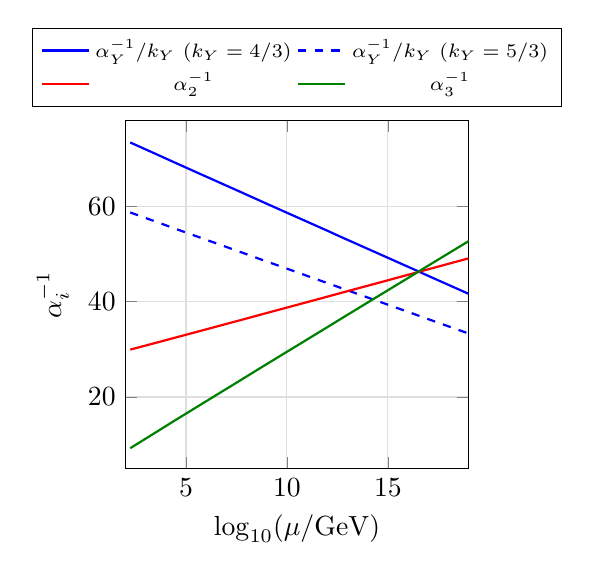
\begin{tikzpicture}
\begin{axis}[width=0.49\textwidth,height=6.0cm,xlabel={$\log_{10}(\mu/\mathrm{GeV})$},ylabel={$\alpha_i^{-1}$},
 legend style={font=\scriptsize,at={(0.5,1.04)},anchor=south,legend columns=2},xmin=2,xmax=19,ymin=5,ymax=78,grid=major,grid style={gray!25}]
\addplot[thick,blue] coordinates {(2.24,73.41) (2.94,72.08) (3.64,70.75) (4.33,69.42) (5.03,68.09) (5.73,66.76) (6.43,65.44) (7.13,64.11) (7.83,62.79) (8.52,61.47) (9.22,60.14) (9.92,58.82) (10.62,57.50) (11.32,56.18) (12.02,54.86) (12.71,53.53) (13.41,52.21) (14.11,50.89) (14.81,49.57) (15.51,48.25) (16.21,46.93) (16.90,45.61) (17.60,44.29) (18.30,42.97) (19.00,41.65)};
\addplot[thick,blue,dashed] coordinates {(2.24,58.73) (2.94,57.66) (3.64,56.60) (4.33,55.53) (5.03,54.47) (5.73,53.41) (6.43,52.35) (7.13,51.29) (7.83,50.23) (8.52,49.17) (9.22,48.11) (9.92,47.06) (10.62,46.00) (11.32,44.94) (12.02,43.88) (12.71,42.83) (13.41,41.77) (14.11,40.71) (14.81,39.66) (15.51,38.60) (16.21,37.55) (16.90,36.49) (17.60,35.43) (18.30,34.38) (19.00,33.32)};
\addplot[thick,red] coordinates {(2.24,29.95) (2.94,30.73) (3.64,31.52) (4.33,32.31) (5.03,33.10) (5.73,33.89) (6.43,34.69) (7.13,35.49) (7.83,36.28) (8.52,37.08) (9.22,37.88) (9.92,38.68) (10.62,39.48) (11.32,40.28) (12.02,41.08) (12.71,41.88) (13.41,42.68) (14.11,43.48) (14.81,44.28) (15.51,45.09) (16.21,45.89) (16.90,46.69) (17.60,47.49) (18.30,48.30) (19.00,49.10)};
\addplot[thick,green!50!black] coordinates {(2.24,9.26) (2.94,11.10) (3.64,12.94) (4.33,14.77) (5.03,16.59) (5.73,18.41) (6.43,20.23) (7.13,22.04) (7.83,23.86) (8.52,25.67) (9.22,27.48) (9.92,29.29) (10.62,31.09) (11.32,32.90) (12.02,34.71) (12.71,36.51) (13.41,38.31) (14.11,40.12) (14.81,41.92) (15.51,43.72) (16.21,45.52) (16.90,47.32) (17.60,49.12) (18.30,50.92) (19.00,52.72)};
\legend{{$\alpha_Y^{-1}/k_Y$ ($k_Y=4/3$)},{$\alpha_Y^{-1}/k_Y$ ($k_Y=5/3$)},{$\alpha_2^{-1}$},{$\alpha_3^{-1}$}}
\end{axis}
\end{tikzpicture}\hfill
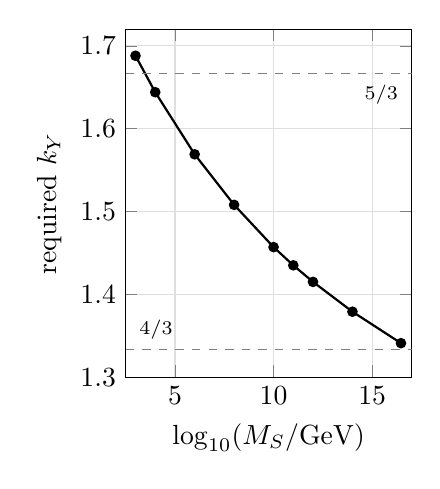
\begin{tikzpicture}
\begin{axis}[width=0.43\textwidth,height=6.0cm,xlabel={$\log_{10}(M_S/\mathrm{GeV})$},ylabel={required $k_Y$},
 xmin=2.5,xmax=17,ymin=1.3,ymax=1.72,grid=major,grid style={gray!25},legend style={font=\scriptsize}]
\addplot[thick,black,mark=*,mark size=1.5pt] coordinates {(3,1.688) (4,1.644) (6,1.569) (8,1.508) (10,1.457) (11,1.435) (12,1.415) (14,1.379) (16.46,1.341)};
\addplot[dashed,gray] coordinates {(2.5,1.6667) (17,1.6667)};
\addplot[dashed,gray] coordinates {(2.5,1.3333) (17,1.3333)};
\node[font=\scriptsize,anchor=north east] at (axis cs:16.8,1.665) {$5/3$};
\node[font=\scriptsize,anchor=south west] at (axis cs:2.7,1.334) {$4/3$};
\end{axis}
\end{tikzpicture}
\caption{Left: two-loop running of the Standard Model couplings; the hypercharge coupling is shown with the canonical
normalisation $\kY=5/3$ (dashed) and with $\kY=4/3$ (solid). Right: the value of $\kY$ required for exact unification when the
MSSM replaces the Standard Model above a scale $M_S$; the last point is the pure Standard Model (script~09).}\label{fig:run}
\end{figure}

\subsection{Where can \texorpdfstring{$\kY=4/3$}{kY = 4/3} come from? (script 06)}

\paragraph{Schellekens' theorem.} In weakly coupled heterotic models with $SU(3)$ and $SU(2)$ at level one, the absence of
fractionally charged states requires $k_3/3+k_2/4+\kY/4\in\mathbb Z$, hence $\kY\ge5/3$ \cite{Schellekens,DFMR,DienesReview}.
Any $\kY<5/3$ therefore implies fractional electric charges. We implemented the generalised condition of \cite{DFMR}: charges
quantised in units of $1/p$ are possible iff
$[p\not\equiv0\ (3)]/3+[p\not\equiv0\ (2)]/4+p^2\kY/4\in\mathbb Z$. The minimal $p$ is
\begin{center}\begin{tabular}{lccccc}\toprule
$\kY$ & $5/3$ & $\mathbf{4/3}$ & $5/4$ & $32/25$ & $13/10$\\\midrule
minimal charge unit & $1$ & $\mathbf{1/6}$ & $1/12$ & $1/30$ & $1/60$\\\bottomrule
\end{tabular}\end{center}
Within $1.31\le\kY\le1.37$ the only values reachable with $p\le6$ are $4/3$ ($p=6$) and $101/75$ ($p=5$).
\emph{$4/3$ is the least exotic candidate}: it needs only sixths, the unit already present in quark hypercharges.

\paragraph{Embeddings.} For $U(1)_Y\subset SU(N)$ with fundamental $(3,1)_a+(1,2)_b+$singlets, $\kY=2\,\mathrm{tr}\,Y^2$. $SU(5)$
is rigid ($5/3$). $SU(6)$ is not: requiring only that $t^c$ sit in the adjoint leaves $\kY(a)=24a^2-8a+4/3$. But
$Y=\mathrm{diag}(\tfrac13,\tfrac13,\tfrac13,-\tfrac13,-\tfrac13,-\tfrac13)$, the generator used in the seven-dimensional
orbifold model of \cite{BJLL2}, is the point of \emph{enhanced symmetry} of that family: it commutes with
$SU(3)\times SU(3)\subset SU(6)$. It gives $\sin^2\theta_W(\MU)=1/(1+\kY)=3/7$ instead of $3/8$. Enumerating
hypercharge generators with entries in $\frac1{12}\mathbb Z$ and at least one Standard Model field in the adjoint yields
23 distinct $\kY$ in $SU(6)$ and 165 in $SU(7)$, of which exactly one, $4/3$, falls in the window.

\paragraph{A cross-check between frameworks.} In that $SU(6)$ model the fundamental contains a doublet $(1,2)_{-1/3}$ with
electric charges $1/6$ and $-5/6$: precisely the unit demanded by the Schellekens condition for $\kY=4/3$, although the two
frameworks (field theory on an orbifold; world-sheet conformal field theory) are independent. Physically, the heavy
$(3,2)_{2/3}$ gauge bosons carry charges $7/6$ and $1/6$ and cannot decay into Standard Model particles: no gauge-mediated
proton decay, but stable fractionally charged relics near $\MU$.

\paragraph{Two negative results.} (a) The weakly coupled heterotic string is the most rigid architecture, since
$M_{\rm string}=5.27\times10^{17}g_{\rm string}\GeV$ \cite{Kaplunovsky} leaves a single continuous parameter. Fitting it to
$\alpha_3$ at two loops gives $g_{\rm string}=0.508$, $M_{\rm string}=2.7\times10^{17}\GeV$ and $\ainv(0)=143.8$ ($+4.9\%$) for
$\kY=4/3$, $160.0$ for $5/3$: the familiar string-scale/unification-scale mismatch, seen from the side of $\alpha$.
(b) Intersecting-brane models have no $\kY$ but linear relations at the string scale. The relation
$\ainv_Y=\tfrac23\ainv_3+\ainv_2$ \cite{BLS} is satisfied by the Standard Model at $4.7\times10^{13}\GeV$; the variant
$\ainv_Y=\tfrac23\ainv_3+\tfrac12\ainv_2$ \cite{KokorelisLike} at $1.4\times10^{18}\GeV$, which with $M_s$ set to the reduced Planck
mass would give $\ainv(0)=138.3$. With two relations and four reference scales tried, one $1\%$ agreement has a chance
probability of order $40\%$: not significant.

%======================================================================
\section{Stress tests}
%======================================================================

\subsection{Kaluza--Klein thresholds of the \texorpdfstring{$SU(6)$}{SU(6)} model (script 07)}
The model is a 7D supersymmetric $SU(6)$ gauge theory on $M^4\times T^2/Z_6\times S^1/Z_2$; in 4D language, $V+\Sigma_{1,2,3}$ in
the adjoint, with the $Z_6$ phases and $Z_2$ parities of \cite{BJLL2}. Two counting rules suffice: on $T^2/Z_6$ each orbit of six
non-zero momenta yields one mode for \emph{every} $Z_6$ charge, while the zero-momentum mode needs trivial charge; on $S^1/Z_2$
even fields have $n\ge0$ and odd fields $n\ge1$. The script reproduces the zero modes stated in the paper (Standard Model gauge
bosons, a $U(1)'$ and $t^c$), which validates the counting, and gives per level
\begin{center}\begin{tabular}{lll}\toprule
Tower & $(b_Y,b_2,b_3)$ & nature\\\midrule
(i) $p=0$, $n\ge1$ & $(8/3,-4,-5)$ & massive vectors and one $(3,1)_{2/3}$ hypermultiplet\\
(ii) $p\ne0$, $n=0$ & $(-16/3,-8,-8)$ & $N{=}2$ multiplets of $SU(5)\times U(1)'$: the 6D fixed planes\\
(iii) $p\ne0$, $n\ge1$ & $(0,0,0)$ & complete $N{=}4$ multiplets\\\bottomrule
\end{tabular}\end{center}
Tower (ii) respects $SU(5)\times U(1)'$, not $SU(6)$. It is universal for $SU(2)$ and $SU(3)$ ($b=-8$, the value expected for
$N{=}2$ $SU(5)$ with two fundamental hypermultiplets) but not for hypercharge, which mixes $SU(5)$ with $U(1)'$:
$b_Y/\kY=-4\ne-8$. Its number of levels grows like $(\Lambda R)^2$. \emph{The relation $\kY=4/3$ thus receives a non-universal,
power-law correction} and is protected only if the cutoff is close to the compactification scale. An observer extrapolating the
Standard Model to the crossing $\alpha_2=\alpha_3$ would measure
\begin{equation}
\kY^{\rm apparent}-\tfrac43\simeq0.018\,S_1+0.018\,S_2,\qquad S_1=\sum_{n<\Lambda R'}\ln\frac{\Lambda R'}{n},\quad
S_2=\sum_{\text{orbits},\,|p|<\Lambda}\ln\frac{\Lambda}{|p|}.
\end{equation}
The sign is the right one, and the required $+0.0077\pm0.0038$ is obtained for $\Lambda R\simeq1.2$--$1.5$: the residual
$0.36$ units come out without tuning. But at $2\sigma$ one needs $\Lambda R\le2.25$ and $\Lambda R'\le2.15$, whereas naive
dimensional analysis puts 7D strong coupling near $\Lambda R\simeq17$.

\paragraph{Literature check.} That loops on orbifolds generate gauge kinetic terms localised on fixed loci, with coefficients set by
the reduced local symmetry, is established \cite{GNH1,GNH2,GLS,Lee6D}. In all cases treated there the fixed loci are points, the
localised terms diverge logarithmically, and the power-like corrections are universal bulk effects which, as noted in \cite{Lee6D}, leave unification untouched. The 7D construction differs because $S^1/Z_2$ creates codimension-one fixed planes, on which a localised
kinetic term diverges quadratically; tower (ii) is exactly that. We found no threshold calculation for this model
(its authors note that 7D orbifold breakings had not been studied before). Related string-based bounds on the ratio of cutoff to
compactification scale exist \cite{HT}. Status: a simple corollary of established principles, apparently not written down for this
geometry, not contradicted, \emph{not verified by a specialist}, and computed with a supersymmetric Kaluza--Klein spectrum
(Scherk--Schwarz splittings ignored).

\paragraph{Relics.} The lightest fractionally charged states have $M\simeq1/R\simeq2\times10^{16}\GeV$. Thermal production stays below
the dark-matter density for $T_{\max}<M/28$ and below $10^{-10}$ of it for $T_{\max}<M/40\simeq5\times10^{14}\GeV$, compatible with
current bounds on the scale of inflation. No cosmological obstacle, and no expected signal.

\subsection{Bayesian evidence with an explicit Occam penalty (script 09)}
We computed $Z=\int\pi(\theta)L(\theta)\,d\theta$ in the Laplace approximation at two loops, with a Gaussian theoretical error
$\sigma$ per coupling and flat priors ($\ln M\in[1\TeV,\MPl]$, $\ainv_U\in[0,100]$, $\kY\in[1,2]$ when free).

\begin{table}[h]\centering
\caption{Evidence of the architectures for $\sigma=0.5$ (script 09). The ranking is unchanged for $\sigma=1$.}\label{tab:bayes}
\begin{tabular}{lccc}\toprule
Architecture & $\chi^2_{\min}$ & $\ln Z$ & Bayes factor\\\midrule
MSSM at $3\TeV$, $\kY=5/3$ & 0.00 & $-9.53$ & 1\\
SM, $\kY=4/3$ & 0.02 & $-9.63$ & 0.91\\
SM, $\kY=13/10$ & 0.57 & $-9.89$ & 0.70\\
SM, $\kY=32/25$ & 1.28 & $-10.24$ & 0.49\\
MSSM, $M_S$ free, $\kY=5/3$ & 0.00 & $-10.70$ & 0.31\\
SM, $\kY$ free (continuous) & 0.00 & $-11.60$ & 0.13\\
rigid strong coupling (family of Table~\ref{tab:scan}, one loop) & -- & $-13.5$ & 0.02\\
SM, $\kY=5/3$ & 27.7 & $-23.6$ & $8\times10^{-7}$\\
weakly coupled heterotic, $\kY=4/3$ & 49.1 & $-30.9$ & $5\times10^{-10}$\\\bottomrule
\end{tabular}\end{table}

``Standard Model $+\,4/3$'' and ``MSSM at $3\TeV+5/3$'' tie. Making $\kY$ continuous costs a factor of seven, which puts a
number on the value of a discrete datum. But the fit alone does \emph{not} select $4/3$ over $13/10$ or $32/25$ once unknown
thresholds are allowed for: what singles out $4/3$ is the structural argument above, not the statistics.

\subsection{Degeneracy with the supersymmetry scale}\label{sec:degeneracy}
If the MSSM replaces the Standard Model above $M_S$, the required $\kY$ moves continuously from $1.688$ ($M_S=1\TeV$) through
$1.457$ ($10^{10}\GeV$) to $1.341$ (no supersymmetry), see Fig.~\ref{fig:run}. The two known solutions, $5/3$ with supersymmetry
at a few TeV and $4/3$ with a desert, are the two ends of one line. This is the conservation lemma again: the discrete ($\kY$)
is exchanged for the continuous ($M_S$). The conclusion ``$\kY=4/3$'' holds \emph{under the desert hypothesis}.

\subsection{The Higgs quartic coupling as an independent observable}
With approximate NLO running, $\lambda(\MU)=-0.0152$ for $M_t=173.34\GeV$ ($-0.0112$ for $172.70$, $-0.0028$ for $171.34$),
and $\lambda$ vanishes near $4\times10^{9}$--$2\times10^{10}\GeV$; requiring $\lambda(\MU)\ge0$ would need $M_h\gtrsim130\GeV$, in
agreement with the stability bound of \cite{Degrassi,Buttazzo}, which serves as a check of the code. In the $SU(6)$ model
supersymmetry is broken at the compactification scale, which imposes at tree level
$0\le\lambda(\MU)\le(g_2^2+g_Y^2)/8=0.060$. The extrapolated value lies outside this window. A loop-sized negative threshold
$\delta\lambda\simeq-0.01$ would cure it, so this is a tension and not an exclusion; and placing supersymmetry where $\lambda$
vanishes gives $\kY\simeq1.46$, no longer $4/3$.

%======================================================================
\section{Scorecard: what was recovered, and how}\label{sec:score}
%======================================================================

\begin{table}[h]\centering\small
\caption{Established results recovered during the session.}\label{tab:score}
\begin{tabular}{>{\raggedright}p{4.1cm}>{\raggedright}p{3.0cm}>{\raggedright\arraybackslash}p{7.9cm}}\toprule
Known result & Source & Route taken here\\\midrule
Running of $\alpha$, infrared floor & textbook & recalled; used as a constraint (Wyler above the floor)\\
Wyler's formula; ``numerology'' critique & \cite{Wyler,Robertson} & recovered as the unique $10^{-6}$ hit of a 5.8-million class; critique \emph{quantified} with decoys\\
Induced QED gives the right order of magnitude & \cite{Landau,Zeldovich} & redone with hypercharge above $M_Z$: 82 vs.\ 137; rephrased as a spectral budget\\
Strong unification / universal Landau pole & \cite{MPP,GLR,ULP} & emerged from a blind scan of 151{,}263 spectra ($n_5+3n_{10}=6$--$7$)\\
SM unifies for $\kY=4/3$ at two loops & \cite{BJLL1,BJLL2} & independent inputs \cite{Buttazzo}; expressed as a prediction $\ainv(0)=136.7$\\
MSSM unification prefers $M_S$ of a few TeV & standard & appears as $\kY^{\rm req}=5/3$ at $M_S\simeq3\TeV$ on a continuous curve\\
$\kY<5/3$ implies fractional charges & \cite{Schellekens,DFMR} & generalised condition coded; $p=6$ for $4/3$; matched to the $SU(6)$ exotics\\
String-scale vs.\ unification-scale mismatch & \cite{Kaplunovsky,DienesReview} & one-parameter two-loop fit: $\ainv(0)=143.8$\\
Brane relation among couplings & \cite{BLS} & tested on the SM; chance probability estimated\\
Localised kinetic terms on orbifolds & \cite{GNH1,GNH2,GLS,Lee6D} & extended by mode counting to codimension-one fixed planes\\
Vacuum stability bound $M_h\gtrsim129$--$130\GeV$ & \cite{Degrassi,Buttazzo} & reproduced ($130.0$) with a simplified NLO code\\\bottomrule
\end{tabular}\end{table}

Items that, to our knowledge, are not in the literature in this form, and which should be treated with corresponding caution:
the above-the-floor argument against Wyler; the decoy-based statistics of volume formulae; the conservation lemma as stated;
the match between the generalised Schellekens unit $1/6$ and the $SU(6)$ orbifold exotics; and the non-universal power-law
threshold of Section~6.1.

%======================================================================
\section{What the dialogue did well, and what it got wrong}
%======================================================================

\paragraph{Errors and retractions (in chronological order).}
\begin{enumerate}\itemsep1pt
\item The first system presented $\alpha=Z_0/2R_K$ as relocating the mystery into the vacuum impedance. The second system showed it
to be a tautology. Conceded.
\item ``$\alpha(0)$ depends on all charged masses'' was loosely stated; corrected to the input/relation distinction of Section~2.
\item The first system quoted a Landau pole near $10^{34}\GeV$, then $10^{40}$, then computed $10^{41}\GeV$ for hypercharge; the
factor $1.7$ was unaffected, but the drift was flagged to the user when it was noticed.
\item The near-alignment $(8.84,7.88,8.35)$ noted by the second system was shown by the first to disappear in $SU(5)$
normalisation, $(5.31,7.88,8.35)$, and to be incompatible with complete multiplets; later it was traced to the known
near-unification with $\kY\simeq1.3$.
\item A one-loop preference for $\kY=32/25$ was overturned by the two-loop calculation.
\item A $p\simeq1$--$5\%$ ``signal'' at the Planck scale was reported, explained, and then dissolved by the two-scale scan. In
the first run the decoys had been evaluated on a coarser grid than the real world, which biased the comparison; this was
noticed and rerun before any conclusion was drawn.
\item A proposed example of a hidden sector generating the hierarchy ($SU(3)$ with 16 flavours) was discarded by the first system
itself before being shown, because that theory sits in the conformal window.
\end{enumerate}

\paragraph{What worked.} (a) \emph{Decoys everywhere}: every coincidence was compared with what fictitious targets achieve.
(b) \emph{A price for every continuous parameter}. (c) \emph{Refusing to scan} when the theoretical error exceeds the spacing of
candidates. (d) \emph{Validation by rediscovery}: a search that finds Wyler, or strong unification, without being told, earns some
trust for its null results. (e) \emph{Cross-criticism}: the second system's review produced the best single argument of the
study and removed two misleading statements; the first system's check of that review caught a normalisation artefact and a
hidden parameter. Neither system alone would have produced the same document.

\paragraph{What did not.} The dialogue reproduced the consensus of the field and did not go beyond it. When asked whether it
was worth continuing, the first system answered that further exploration was not: the remaining steps (heterotic M-theory, the
quartic threshold with Scherk--Schwarz breaking, a full NNLO Higgs analysis) require specialist machinery in which its errors
would no longer be detectable by either participant.

%======================================================================
\section{Limitations}\label{sec:limits}
%======================================================================
\begin{itemize}\itemsep1pt
\item One- and two-loop running only; unification-scale thresholds unknown; the conversion of $\alpha_Y(M_t)$ into $\alpha(0)$
is first order.
\item The two-loop terms of the top Yukawa and Higgs quartic equations in script~09 are the leading ones, written from the
model's memory and validated only by the agreement of the resulting stability bound with the literature.
\item Decoy $p$-values depend on the chosen family of representations and multiplicity bounds; the two-scale test used only 16 decoys.
\item The Kaluza--Klein analysis assumes a supersymmetric spectrum and a hard cutoff, and ignores tree-level localised terms.
\item Bibliographic details marked $^\dagger$ in the reference list were recalled from memory and not re-verified online; the
others were checked through web search during the session.
\item The three-hour figure is wall-clock time reported by the human participants, not measured by the AI system.
\end{itemize}

%======================================================================
\section{Conclusion}
%======================================================================
The fine-structure constant is very probably not a direct geometric invariant. It remains plausible that $\alpha(0)$ is the
output of a renormalisation-group calculation whose ultraviolet inputs are discrete. The conclusion of this exercise is conditional:
\begin{quote}
\emph{If} nothing exists between the electroweak scale and $3\times10^{16}\GeV$, \emph{then} the measured couplings require
$\kY=4/3$, a value with an identifiable geometric origin (the $U(1)$ commuting with $SU(3)\times SU(3)$ in $SU(6)$) and a
definite physical price (superheavy stable states with charges in units of $1/6$). In that world the geometric part of
``why 137'' is ``why that embedding''; the unified coupling $\ainv_U\simeq46$ is a moduli-stabilisation problem, and the last
nine units are set by the light spectrum.
\end{quote}
Gauge couplings alone cannot distinguish that world from one with supersymmetry at a few TeV. Proton decay (absent for
$4/3$ in this construction, expected for $5/3$), superpartner searches and sharper top and Higgs masses can.

As an experiment, the outcome is that a steered dialogue between AI systems with a code sandbox can, within an afternoon,
retrace a good part of a thirty-year literature by partly independent routes, attach error bars to its own enthusiasm, and
recognise where it should stop. It did not find anything a specialist would call new, and it said so.

\section*{Author contributions and disclosure}
Fable5.1 wrote and ran all scripts, performed the literature checks and drafted this text, including this sentence.
GPT5.6-Sol contributed the critical review integrated in Sections~2--5 (the tautology of $Z_0/2R_K$, the input status of $\alpha(0)$,
the above-the-floor argument, the spectral budget and its toy solutions, the three-coupling pole condition, the unification and
duality architectures, the precision wall, and the proposal to scan spectra with a parameter penalty).
l0d0v1c and pseudoLuc asked the questions, relayed material between the two systems, chose the follow-ups and kept the time.
No part of this manuscript has been peer reviewed.

%======================================================================
\begin{thebibliography}{99}\small
\bibitem{Eddington} A.~S.~Eddington, \emph{Fundamental Theory}, Cambridge University Press (1946).$^\dagger$
\bibitem{Wyler} A.~Wyler, C.~R.~Acad.~Sci.~Paris \textbf{269A} (1969) 743.$^\dagger$
\bibitem{Robertson} B.~Robertson, Phys.~Rev.~Lett.~\textbf{27} (1971) 1545.$^\dagger$
\bibitem{Hua} L.~K.~Hua, \emph{Harmonic Analysis of Functions of Several Complex Variables in the Classical Domains}, AMS (1963).$^\dagger$
\bibitem{CODATA} CODATA 2022 recommended values of the fundamental physical constants, NIST.
\bibitem{Landau} L.~D.~Landau, in \emph{Niels Bohr and the Development of Physics}, Pergamon (1955).$^\dagger$
\bibitem{Zeldovich} Ya.~B.~Zeldovich, JETP Lett.~\textbf{6} (1967) 345.$^\dagger$
\bibitem{MPP} L.~Maiani, G.~Parisi, R.~Petronzio, Nucl.~Phys.~B\textbf{136} (1978) 115.
\bibitem{GLR} D.~Ghilencea, M.~Lanzagorta, G.~G.~Ross, ``Strong unification'', hep-ph/9707462; ``Unification predictions'', hep-ph/9707401.
\bibitem{ULP} ``Universal Landau pole and physics below the 100 TeV scale'', arXiv:1705.09716.
\bibitem{BJLL1} V.~Barger, J.~Jiang, P.~Langacker, T.~Li, ``Gauge coupling unification in the Standard Model'', Phys.~Lett.~B\textbf{624} (2005) 233, hep-ph/0503226.
\bibitem{BJLL2} V.~Barger, J.~Jiang, P.~Langacker, T.~Li, ``Non-canonical gauge coupling unification in high-scale supersymmetry breaking'', Nucl.~Phys.~B\textbf{726} (2005) 149, hep-ph/0504093.
\bibitem{Buttazzo} D.~Buttazzo, G.~Degrassi, P.~P.~Giardino, G.~F.~Giudice, F.~Sala, A.~Salvio, A.~Strumia, ``Investigating the near-criticality of the Higgs boson'', JHEP \textbf{12} (2013) 089, arXiv:1307.3536.
\bibitem{MV} M.~E.~Machacek, M.~T.~Vaughn, Nucl.~Phys.~B\textbf{222} (1983) 83; B\textbf{236} (1984) 221; B\textbf{249} (1985) 70.
\bibitem{Schellekens} A.~N.~Schellekens, ``Electric charge quantization in string theory'', Phys.~Lett.~B\textbf{237} (1990) 363.
\bibitem{DFMR} K.~R.~Dienes, A.~E.~Faraggi, J.~March-Russell, ``String unification, higher-level gauge symmetries, and exotic hypercharge normalizations'', hep-th/9510223.
\bibitem{DienesReview} K.~R.~Dienes, ``String theory and the path to unification'', Phys.~Rept.~\textbf{287} (1997) 447, hep-th/9602045.
\bibitem{Kaplunovsky} V.~S.~Kaplunovsky, Nucl.~Phys.~B\textbf{307} (1988) 145.$^\dagger$
\bibitem{BLS} R.~Blumenhagen, D.~L\"ust, S.~Stieberger, ``Gauge unification in supersymmetric intersecting brane worlds'', JHEP \textbf{07} (2003) 036, hep-th/0305146.
\bibitem{KokorelisLike} ``$N=1$ locally supersymmetric Standard Models from intersecting branes'', hep-th/0309070, eq.~(7.9).
\bibitem{GNH1} S.~Groot Nibbelink, M.~Hillenbach, hep-th/0503153.$^\dagger$
\bibitem{GNH2} S.~Groot Nibbelink, M.~Hillenbach, hep-th/0602155.$^\dagger$
\bibitem{GLS} D.~M.~Ghilencea, H.~M.~Lee, K.~Schmidt-Hoberg, ``Higher derivatives and brane-localised kinetic terms in gauge theories on orbifolds'', hep-ph/0604215.
\bibitem{Lee6D} H.~M.~Lee, ``Gauge coupling unification in six dimensions'', hep-ph/0611196.
\bibitem{HT} A.~Hebecker, M.~Trapletti, ``Gauge unification in highly anisotropic string compactifications'', hep-th/0411131.$^\dagger$
\bibitem{Degrassi} G.~Degrassi, S.~Di~Vita, J.~Elias-Mir\'o, J.~R.~Espinosa, G.~F.~Giudice, G.~Isidori, A.~Strumia, ``Higgs mass and vacuum stability in the Standard Model at NNLO'', JHEP \textbf{08} (2012) 098, arXiv:1205.6497.
\end{thebibliography}

\appendix
%======================================================================
\section{Methods}
%======================================================================
\paragraph{Volumes.} Hua's volumes of the classical domains and of the auxiliary spaces are
\begin{align*}
V(\mathrm{I}_{m,n})&=\pi^{mn}\,\frac{\prod_{j<m}j!\,\prod_{j<n}j!}{\prod_{j<m+n}j!}, &
V(\mathrm{II}_n)&=\frac{\pi^{n(n+1)/2}}{2^{n(n-1)/2}}\,\frac{\prod_{k<n}(2k)!}{\prod_{k=n}^{2n-1}k!},\\
V(\mathrm{III}_n)&=\pi^{n(n-1)/2}\,\frac{\prod_{k<n-1}(2k)!}{\prod_{k=n-1}^{2n-3}k!}, &
V(\mathrm{IV}_n)&=\frac{\pi^n}{2^{n-1}n!},\\
V(Q^n)&=\frac{2\pi^{n/2+1}}{\Gamma(n/2)}, & V(S^k)&=\frac{2\pi^{(k+1)/2}}{\Gamma((k+1)/2)} .
\end{align*}
Values are handled as
logarithms, deduplicated at $10^{-11}$ and searched by bisection. Domain normalisations are conventional (e.g.\ I$(2,2)$ and IV$(4)$
describe the same space and differ by a factor 16), which is itself an argument against a direct physical reading.

\paragraph{Spectra.} One-loop contributions per vector-like Dirac fermion, convention $Q=T_3+Y$: $E\,(\tfrac43,0,0)$, $L\,(\tfrac23,\tfrac23,0)$,
$D\,(\tfrac49,0,\tfrac23)$, $U\,(\tfrac{16}9,0,\tfrac23)$, $Q\,(\tfrac29,2,\tfrac43)$, real $T\,(0,\tfrac43,0)$, real $G\,(0,0,2)$; supersymmetric
version $\times\tfrac32$. $b^{\rm SM}=(\tfrac{41}6,-\tfrac{19}6,-7)$, $b^{\rm MSSM}=(11,1,-3)$. Feasibility of
$0\le\ainv_i(M_Z)-[b_i\ln(\Lambda/M_Z)+\Delta b_i\ln(\Lambda/M)]/2\pi\le1$ is decided by scanning $\ln\Lambda$ and intersecting intervals in
$\ln(\Lambda/M)$. Inputs at $M_Z$: $\ainv=127.951$, $\sin^2\theta_W=0.23122$, $\alpha_s=0.1180$.

\paragraph{Two-loop running.} Runge--Kutta integration of the gauge equations with
$b=(\tfrac{41}{10},-\tfrac{19}6,-7)$ and the standard two-loop matrix in $SU(5)$ normalisation, top Yukawa at one loop, from the
couplings of \cite{Buttazzo} at $M_t=173.34\GeV$. MSSM coefficients from \cite{BJLL2}, $\tan\beta=10$, no $\overline{\rm MS}$--$\overline{\rm DR}$ conversion.

\paragraph{Evidence.} Laplace approximation,
$\ln Z=-\tfrac12\chi^2_{\min}+\tfrac{m-n}2\ln(2\pi\sigma^2)-\tfrac12\ln\det(J^{\!\top}J)-\ln V_{\rm prior}$ with $n=3$ observables, $m$ parameters
and $J$ the Jacobian at the best fit.

%======================================================================
\section{Python sources}
%======================================================================
All scripts require only Python~3 and \texttt{numpy}. Long lines are wrapped for display (marked $\hookrightarrow$); the code is
otherwise reproduced verbatim from the files that produced the numbers in this paper. Indicative run times on a single core:
scripts 01, 04, 07: seconds; 02, 05: about a minute; 06, 09: two to three minutes; 03 and 08: several minutes, proportional to the
number of decoy worlds requested on the command line.

\subsection{\texttt{01\_wyler.py}}
Wyler's formula in dimension $n$ and brute-force search (Section 3.3).
\begin{lstlisting}
#!/usr/bin/env python3
"""
01 - Wyler's formula: generalisation to dimension n, and brute-force search
     in the class 2^a 3^b 5^c pi^d (quarter-integer exponents).
"""
import numpy as np, math
from math import pi, gamma, factorial

T = 137.035999177                      # 1/alpha, CODATA 2022

def VD(n): return pi**n/(2**(n-1)*factorial(n))          # Cartan domain of type IV (Hua)
def VQ(n): return 2*pi**(n/2+1)/gamma(n/2)               # Shilov boundary Q^n
def VS(k): return 2*pi**((k+1)/2)/gamma((k+1)/2)         # sphere S^k

print("== Wyler in dimension n:  alpha = 3 V(S^{n-1}) / V(Q^n)^2 * V(D^n)^(1/4) ==")
for n in range(3, 9):
    a = VS(n-1)/VQ(n)*(3/VQ(n))*VD(n)**0.25
    print(f"  n = {n}   1/alpha = {1/a:.5f}")
print("  closed form n=5:", 2**4.75*3**-1.75*5**.25*pi**2.75)

print("\n== Brute-force search 2^a 3^b 5^c pi^d, exponents multiples of 1/4 ==")
L = [math.log(x) for x in (2, 3, 5, pi)]; lt = math.log(T)
for R in (8, 16, 24):                                    # exponents in [-R/4, R/4]
    e = np.arange(-R, R+1)/4
    s01 = (e[:,None]*L[0] + e[None,:]*L[1]).ravel()
    s23 = np.sort((e[:,None]*L[2] + e[None,:]*L[3]).ravel())
    for tol in (1e-6, 1e-7, 1e-8):
        n = (np.searchsorted(s23, lt-s01+tol) - np.searchsorted(s23, lt-s01-tol)).sum()
        print(f"  |exponent| <= {R/4:.0f}   tolerance {tol:.0e} : {int(n)} formula(e)")
\end{lstlisting}

\subsection{\texttt{02\_cartan\_volumes.py}}
Cartan-volume coincidences with decoy targets (Section 3.3).
\begin{lstlisting}
#!/usr/bin/env python3
"""
02 - Search for coincidences between physical constants and products of volumes
     of symmetric spaces (Cartan domains I-IV, spheres, Shilov boundaries),
     with a look-elsewhere control based on decoy targets.
"""
import numpy as np, itertools
from math import pi, factorial as f, gamma, log

def prod(it):
    r = 1.0
    for x in it: r *= x
    return r

B = {}
for n in range(1, 9):                                            # type IV (Lie balls)
    B[f"IV{n}"] = pi**n/(2**(n-1)*f(n))
for m, n in [(1,2),(1,3),(1,4),(1,5),(2,2),(2,3),(2,4),(3,3)]:   # type I (m,n)
    B[f"I{m}{n}"] = prod(f(k) for k in range(1,m))*prod(f(k) for k in range(1,n)) \
                    / prod(f(k) for k in range(1,m+n)) * pi**(m*n)
for n in (2, 3):                                                 # type II
    B[f"II{n}"] = pi**(n*(n+1)/2)/2**(n*(n-1)/2) \
                  * prod(f(2*k) for k in range(1,n))/prod(f(k) for k in range(n,2*n))
for n in (3, 4, 5):                                              # type III
    B[f"III{n}"] = pi**(n*(n-1)/2) \
                   * prod(f(2*k) for k in range(1,n-1))/prod(f(k) for k in range(n-1,2*n-2))
for k in range(1, 9): B[f"S{k}"] = 2*pi**((k+1)/2)/gamma((k+1)/2)
for n in range(2, 9): B[f"Q{n}"] = 2*pi**(n/2+1)/gamma(n/2)

names = list(B); L = np.array([log(B[k]) for k in names]); nb = len(names)
EXP = np.array([-2, -1, -.5, -.25, .25, .5, 1, 2])
C = {"1":1, "2":2, "3":3, "4":4, "1/2":.5, "1/3":1/3, "1/4":.25, "3/2":1.5, "2/3":2/3}
cn = list(C); lc = np.array([log(v) for v in C.values()])
TARGETS = {"1/alpha":137.035999177, "mp/me":1836.152673426,
           "mmu/me":206.7682827, "mn/me":1838.68366200}       # CODATA 2022
lt = {k: log(v) for k, v in TARGETS.items()}

vals, hits = [], {k: [] for k in TARGETS}
for r in (1, 2, 3):
    for comb in itertools.combinations(range(nb), r):
        v = lc.copy()
        for i in comb: v = v[..., None] + L[i]*EXP
        for k in TARGETS:
            for ix in np.argwhere(np.abs(v-lt[k]) < 1e-6):
                hits[k].append((float(abs(v[tuple(ix)]-lt[k])), comb, tuple(ix)))
        vals.append(v.ravel())
V = np.unique(np.round(np.concatenate(vals), 11))
print(nb, "building blocks;", len(V), "distinct values")

rng = np.random.default_rng(1)
for k in TARGETS:
    print("\n==", k)
    for tol in (1e-5, 1e-6, 1e-7, 1e-8):
        n = np.searchsorted(V, lt[k]+tol) - np.searchsorted(V, lt[k]-tol)
        d = lt[k] + rng.uniform(-.2, .2, 4000)                   # local decoy targets
        nd = np.searchsorted(V, d+tol) - np.searchsorted(V, d-tol)
        print(f"  tol {tol:.0e}: real {n:3d} | decoys, mean {nd.mean():6.2f} | P(decoy >= real) = {np.mean(nd>=n):.2f}")
    for e, comb, ix in sorted(hits[k])[:4]:
        s = cn[ix[0]] + " * " + " * ".join(f"{names[i]}^{EXP[j]:g}" for i, j in zip(comb, ix[1:]))
        print(f"     deviation {e:.1e}:  {s}")
\end{lstlisting}

\subsection{\texttt{03\_spectrum\_scan.py}}
Scan of vector-like spectra with decoy worlds (Section 4.2).
\begin{lstlisting}
#!/usr/bin/env python3
"""
03 - Scan of vector-like spectra: which matter contents make the three gauge couplings
     simultaneously strong (0 <= alpha_i^-1(Lambda) <= 1) at a common scale Lambda?
     One loop, a single common mass M >= 1 TeV. Control: decoy worlds.

Usage: python3 03_spectrum_scan.py [number_of_decoys]   (default 20; 80 were used for the paper,
       allow several minutes per configuration)
"""
import numpy as np, itertools, math, sys
tp = 2*math.pi; MZ = 91.1876
AINV, S2W, AS = 127.951, 0.23122, 0.1180
A = np.array([AINV*(1-S2W), AINV*S2W, 1/AS])          # 1/alpha_Y, 1/alpha_2, 1/alpha_3 at M_Z
bSM = np.array([41/6, -19/6, -7.0]); bMSSM = np.array([11.0, 1.0, -3.0])   # convention Q = T3 + Y
# (db_Y, db_2, db_3) per vector-like Dirac fermion; T and G: real fermions
FIELDS = {"E":(4/3,0,0), "L":(2/3,2/3,0), "D":(4/9,0,2/3), "U":(16/9,0,2/3),
          "Q":(2/9,2,4/3), "T":(0,4/3,0), "G":(0,0,2)}
names = list(FIELDS); C = np.array(list(FIELDS.values()))
S = np.array(list(itertools.product(*[range(7)]*5, range(3), range(3))))
comp = S.sum(1)
su5 = (S[:,1]==S[:,2]) & (S[:,0]==S[:,3]) & (S[:,0]==S[:,4]) & (S[:,5]==0) & (S[:,6]==0)

def feasible(A, susy, xlo, xhi, nx=40, Mmin=1000.):
    """For each spectrum: is there (Lambda, M) such that alpha_i^-1(Lambda) lies in [0,1] for all i?
       x = ln(Lambda/MZ), y = ln(Lambda/M). At fixed x, each coupling imposes an interval in y."""
    db = S@C*(1.5 if susy else 1.0)                    # supermultiplets: x 3/2
    if susy: db = db + (bMSSM - bSM)                   # superpartners at the same scale M
    x = np.linspace(xlo, xhi, nx); ymax = x - math.log(Mmin/MZ)
    lo = np.zeros((len(S), nx)); hi = np.broadcast_to(ymax, (len(S), nx)).copy()
    ok = np.ones((len(S), nx), bool)
    for i in range(3):
        up = tp*A[i] - bSM[i]*x; dn = up - tp          # db_i * y must fall in [dn, up]
        d = db[:, i][:, None]
        with np.errstate(divide='ignore', invalid='ignore'):
            l = np.where(d > 0, dn/d, -np.inf); h = np.where(d > 0, up/d, np.inf)
        ok &= np.where(d > 0, True, (dn <= 0) & (up >= 0))
        lo = np.maximum(lo, l); hi = np.minimum(hi, h)
    f = ok & (lo <= hi); any_ = f.any(1)
    ix = np.where(any_, (f*np.arange(nx)).sum(1)//np.maximum(f.sum(1), 1), 0)
    r = np.arange(len(S))
    return any_, x[ix], (lo[r, ix] + hi[r, ix])/2

if __name__ == "__main__":
    ndec = int(sys.argv[1]) if len(sys.argv) > 1 else 20
    X = lambda lam: math.log(lam/MZ)
    windows = {"Lambda free 1e10 - 1.22e19 GeV": (X(1e10), X(1.22e19), 60),
               "Planck window 2.4e18 - 1.22e19 GeV": (X(2.435e18), X(1.22e19), 30)}
    rng = np.random.default_rng(11)
    print(len(S), "spectra; couplings at M_Z:", np.round(A, 3))
    for susy in (False, True):
        for wn, (a, b, nx) in windows.items():
            ok, xb, yb = feasible(A, susy, a, b, nx)
            print(f"\n### base {'MSSM (superpartners at M)' if susy else 'Standard Model'} | {wn}")
            print(f"  compatible spectra: {ok.sum()} ({100*ok.mean():.2f} %); minimal complexity: {comp[ok].min()}")
            for w in (1.25, 1.5, 2.0):
                dec = A*np.exp(rng.uniform(-math.log(w), math.log(w), (ndec, 3)))
                nd = np.array([feasible(d, susy, a, b, nx)[0].sum() for d in dec])
                print(f"  decoys x{w:<4}: median {np.median(nd):6.0f} | P(decoy >= real) = {np.mean(nd >= ok.sum()):.3f}")
            for j in np.where(ok)[0][np.argsort(comp[ok])][:5]:
                lam = MZ*math.exp(xb[j]); M = lam*math.exp(-yb[j])
                print("    ", {n: int(v) for n, v in zip(names, S[j]) if v}, f"Lambda ~ {lam:.1e}  M ~ {M:.1e} GeV")
            print("   complete SU(5) multiplets (n5, n10):", [(int(S[j][1]), int(S[j][0])) for j in np.where(ok & su5)[0]])
    # test of the interpretation: the excess in the Planck window comes from the near-equality of the required db
    print("\n### 'democracy' test (SM base, Planck window): required R_i = db_i * y")
    a, b, nx = windows["Planck window 2.4e18 - 1.22e19 GeV"]; x0 = (a+b)/2
    print("  real world: R =", np.round(tp*A - bSM*x0, 1))
    for R in [(330,330,330), (420,330,250), (250,330,420), (500,330,160), (160,330,500)]:
        Ad = (np.array(R) + bSM*x0)/tp
        print(f"  R = {R} -> {feasible(Ad, False, a, b, nx)[0].sum()} spectra")
\end{lstlisting}

\subsection{\texttt{04\_strong\_coupling\_prediction.py}}
Prediction of $1/\alpha(0)$ under common strong coupling (Section 4.3).
\begin{lstlisting}
#!/usr/bin/env python3
"""
04 - 'Common strong coupling' scenario: MSSM + n complete SU(5) multiplets (n = n5 + 3 n10)
     at the scale M (superpartners included), alpha_i^-1(Lambda) = c * k_i with c in [0,1].
     Lambda is fitted to alpha_s; alpha_2, alpha_Y, sin^2(theta_W) and 1/alpha(0) are predicted.
     Shows the hypersensitivity to M: d(1/alpha(0))/d ln M ~ 11.   One loop.
"""
import math
tp = 2*math.pi; MZ = 91.1876
A = dict(Y=98.366, w=29.585, s=8.4746)                 # 1/alpha_i(M_Z)
D_IR = 137.035999 - 127.951                            # running from M_Z down to 0
bSM = dict(Y=41/6, w=-19/6, s=-7.0); bMSSM = dict(Y=11.0, w=1.0, s=-3.0)
k = dict(Y=5/3, w=1.0, s=1.0)                          # one complete multiplet: db_i = k_i

print(" n   M(TeV)   c    Lambda(GeV)   1/a_2    1/a_Y    sin2_W   1/alpha(0)")
for n in (5, 6, 7):
    for M in (1e3, 3e3, 1e4, 3e4):
        for c in (0, 0.5, 1):
            t = math.log(M/MZ)
            Bh = {i: bMSSM[i] + n*k[i] for i in A}
            xt = (tp*(A['s'] - c) - bSM['s']*t)/Bh['s']          # ln(Lambda/M) fitted to alpha_s
            p = {i: c*k[i] + (bSM[i]*t + Bh[i]*xt)/tp for i in A}
            am = p['Y'] + p['w']
            print(f" {n}   {M/1e3:5.0f}   {c:3.1f}   {M*math.exp(xt):10.2e}   {p['w']:6.2f}   {p['Y']:6.2f}   {p['w']/am:.4f}   {am + D_IR:8.2f}")
\end{lstlisting}

\subsection{\texttt{05\_kY\_two\_loops.py}}
Two-loop determination of $k_Y$ and prediction of $1/\alpha(0)$ (Section 5.1).
\begin{lstlisting}
#!/usr/bin/env python3
"""
05 - Hypercharge normalisation k_Y and prediction of 1/alpha(0),
     Standard Model only, at one and two loops.

Principle: impose alpha_Y^-1 / k_Y = alpha_2^-1 = alpha_3^-1 = alpha_U^-1 at M_U.
(M_U, alpha_U) are fitted to the measured alpha_2 and alpha_3; alpha_Y is then PREDICTED,
hence 1/alpha(0) as well:  1/alpha(0)_pred = 137.036 + [alpha_Y^-1 pred - alpha_Y^-1 obs](M_t).

Inputs: MS-bar couplings at mu = M_t = 173.34 GeV, extracted at NNLO by
Buttazzo et al., JHEP 12 (2013) 089 [arXiv:1307.3536], eqs (57)-(59):
  g_Y = 0.35830, g_2 = 0.64779, y_t = 0.93690,
  g_3 = 1.1666 + 0.00314*(alpha_s(MZ)-0.1184)/0.0007
Equations: two-loop SM gauge RGEs (Machacek-Vaughn), one-loop top Yukawa.
Internal normalisation: g1^2 = (5/3) g_Y^2 (a computational convention, with no effect on k_Y).
"""
import numpy as np, math
from fractions import Fraction as Fr

MT = 173.34
ALPHA0_INV = 137.035999177
b  = np.array([41/10, -19/6, -7.0])
B  = np.array([[199/50, 27/10, 44/5],
               [9/10,   35/6,  12.0],
               [11/10,  9/2,  -26.0]])
Ct = np.array([17/10, 3/2, 2.0])
K  = 1/(16*math.pi**2)

def beta(y, loops):
    g, yt = y[:3], y[3]
    dg = K*b*g**3
    if loops == 2:
        dg = dg + K*K*g**3*(B@(g**2) - Ct*yt**2)
    dyt = K*yt*(4.5*yt**2 - 17/20*g[0]**2 - 9/4*g[1]**2 - 8*g[2]**2)
    return np.append(dg, dyt)

def run(y0, t0, t1, loops, n=4000):
    """Runge-Kutta 4 from t0 to t1, t = ln(mu/GeV)."""
    y, h = np.array(y0, float), (t1-t0)/n
    for _ in range(n):
        k1 = beta(y, loops); k2 = beta(y+h/2*k1, loops)
        k3 = beta(y+h/2*k2, loops); k4 = beta(y+h*k3, loops)
        y = y + h/6*(k1+2*k2+2*k3+k4)
    return y

ainv = lambda g: 4*math.pi/g**2

def inputs(alpha_s=0.1180, dyt=0.0):
    gY, g2, yt = 0.35830, 0.64779, 0.93690+dyt
    g3 = 1.1666 + 0.00314*(alpha_s-0.1184)/0.0007
    return np.array([math.sqrt(5/3)*gY, g2, g3, yt])

def k_requis(y0, loops):
    """Run the couplings up, find M_U where alpha_2 = alpha_3, return (M_U, alpha_U^-1, required k_Y)."""
    t, y, h = math.log(MT), y0.copy(), 0.05
    while True:
        yn = run(y, t, t+h, loops, n=20)
        if ainv(yn[1]) - ainv(yn[2]) < 0:   # crossing inside [t, t+h]: bisection
            lo, hi = 0.0, h
            for _ in range(40):
                mid = (lo+hi)/2; ym = run(y, t, t+mid, loops, n=20)
                if ainv(ym[1]) - ainv(ym[2]) < 0: hi = mid
                else: lo = mid
            ym = run(y, t, t+lo, loops, n=20)
            aU = ainv(ym[1]); aYinv = (5/3)*ainv(ym[0])
            return math.exp(t+lo), aU, aYinv/aU, ym[3]
        t, y = t+h, yn

def prediction(kY, y0, loops):
    """Fit (M_U, alpha_U) to alpha_2, alpha_3 at M_t by Newton iteration; predict alpha_Y^-1(M_t)."""
    MU, aU, _, ytU = k_requis(y0, loops)
    p = np.array([math.log(MU), aU])
    target = np.array([ainv(y0[1]), ainv(y0[2])])
    def down(p):
        gU = math.sqrt(4*math.pi/p[1])
        gYU = math.sqrt(4*math.pi/(kY*p[1]))
        y = run([math.sqrt(5/3)*gYU, gU, gU, ytU], p[0], math.log(MT), loops, n=3000)
        return y
    for _ in range(12):
        y = down(p); r = np.array([ainv(y[1]), ainv(y[2])]) - target
        if np.abs(r).max() < 1e-10: break
        J = np.zeros((2,2))
        for j, e in enumerate((1e-4, 1e-4)):
            dp = p.copy(); dp[j] += e; yy = down(dp)
            J[:,j] = (np.array([ainv(yy[1]), ainv(yy[2])]) - target - r)/e
        p = p - np.linalg.solve(J, r)
    y = down(p)
    aY_pred = (5/3)*ainv(y[0]); aY_obs = (5/3)*ainv(y0[0])
    return math.exp(p[0]), p[1], ALPHA0_INV + aY_pred - aY_obs

if __name__ == "__main__":
    y0 = inputs()
    print("Inputs at M_t: 1/alpha_Y = %.3f  1/alpha_2 = %.3f  1/alpha_3 = %.3f"
          % ((5/3)*ainv(y0[0]), ainv(y0[1]), ainv(y0[2])))
    print("\n== k_Y required for exact unification ==")
    for loops in (1, 2):
        MU, aU, k, _ = k_requis(y0, loops)
        print(f"{loops} loop(s): M_U = {MU:.3e} GeV   1/alpha_U = {aU:.3f}   k_Y = {k:.4f}")
    print("\n== uncertainties on k_Y at two loops ==")
    k0 = k_requis(y0, 2)[2]
    for lab, yy in [("alpha_s +0.0009", inputs(0.1189)), ("alpha_s -0.0009", inputs(0.1171)),
                    ("y_t +0.005 (~ M_t +1 GeV)", inputs(dyt=0.005))]:
        print(f"  {lab:28s} dk_Y = {k_requis(yy,2)[2]-k0:+.4f}")
    print("\n== prediction of 1/alpha(0) as a function of k_Y ==")
    print(" k_Y        1 loop     2 loops     dev. 2l    M_U (2l)")
    for fr in (Fr(5,3), Fr(4,3), Fr(13,10), Fr(32,25), Fr(5,4), Fr(6,5), Fr(1,1)):
        r1 = prediction(float(fr), y0, 1); r2 = prediction(float(fr), y0, 2)
        print(f" {str(fr):6s}   {r1[2]:9.2f}   {r2[2]:9.2f}   {100*(r2[2]/ALPHA0_INV-1):+6.2f} %   {r2[0]:.2e}")
\end{lstlisting}

\subsection{\texttt{06\_kY\_origin.py}}
Origin of $k_Y=4/3$: Schellekens condition, embeddings, heterotic and brane tests (Section 5.2).
\begin{lstlisting}
#!/usr/bin/env python3
"""
06 - Where can k_Y = 4/3 come from?  Four tests.

 A. Generalised Schellekens condition (heterotic strings, levels k_2 = k_3 = 1):
    electric charges quantised in units of 1/p are possible iff
        [p mod 3 != 0]/3 + [p mod 2 != 0]/4 + p^2 k_Y/4   is an integer.
    (Dienes, Faraggi, March-Russell, hep-th/9510223, eqs 6.30-6.31; p = 1 gives back
     k_3/3 + k_2/4 + k_Y/4 = 0 mod 1, i.e. k_Y >= 5/3.)
 B. Embeddings of U(1)_Y in SU(N): k_Y = 2 tr(Y^2) on the fundamental
    N = (3,1)_a + (1,2)_b + singlets s_j, traceless. Rigid or not?
 C. Weakly coupled heterotic string: M_string = 5.27e17 * g_string GeV (Kaplunovsky),
    a single continuous parameter. Two-loop predictions.
 D. Brane relations (type II) at the string scale:
      (A) 1/alpha_Y = (2/3)/alpha_3 + 1/alpha_2      (Blumenhagen-Lust-Stieberger 2003)
      (B) 1/alpha_Y = (2/3)/alpha_3 + (1/2)/alpha_2  (Pati-Salam-like variant)
    At which scale does the Standard Model satisfy them?
"""
import numpy as np, math, itertools
from fractions import Fraction as Fr
from math import gcd

# ---------- RGE core (identical to script 05) ----------
MT = 173.34; ALPHA0_INV = 137.035999177
b  = np.array([41/10, -19/6, -7.0])
B  = np.array([[199/50, 27/10, 44/5], [9/10, 35/6, 12.0], [11/10, 9/2, -26.0]])
Ct = np.array([17/10, 3/2, 2.0]); K = 1/(16*math.pi**2)
def beta(y):
    g, yt = y[:3], y[3]
    dg = K*b*g**3 + K*K*g**3*(B@(g**2) - Ct*yt**2)
    return np.append(dg, K*yt*(4.5*yt**2 - 17/20*g[0]**2 - 9/4*g[1]**2 - 8*g[2]**2))
def run(y0, t0, t1, n=3000):
    y, h = np.array(y0, float), (t1-t0)/n
    for _ in range(n):
        k1 = beta(y); k2 = beta(y+h/2*k1); k3 = beta(y+h/2*k2); k4 = beta(y+h*k3)
        y = y + h/6*(k1+2*k2+2*k3+k4)
    return y
ainv = lambda g: 4*math.pi/g**2
g3 = 1.1666 + 0.00314*(0.1180-0.1184)/0.0007
Y0 = np.array([math.sqrt(5/3)*0.35830, 0.64779, g3, 0.93690])       # couplings at M_t
obs = np.array([(5/3)*ainv(Y0[0]), ainv(Y0[1]), ainv(Y0[2])])       # 1/alpha_Y, 1/alpha_2, 1/alpha_3

# ---------- A. generalised Schellekens condition ----------
def ok(p, k): return ((Fr(1,3) if p % 3 else 0) + (Fr(1,4) if p % 2 else 0) + Fr(p*p)*k/4).denominator == 1
def pmin(k, pmax=200):
    return next((p for p in range(1, pmax+1) if ok(p, k)), None)
print("== A. Minimal charge unit 1/p required by k_Y (heterotic, level 1) ==")
for k in (Fr(5,3), Fr(4,3), Fr(13,10), Fr(32,25), Fr(5,4), Fr(7,6), Fr(1)):
    print(f"   k_Y = {str(k):6s}  ->  p_min = {pmin(k)}")
lo, hi = Fr(131,100), Fr(137,100)
print(f"   k_Y allowed in the window [{float(lo)}, {float(hi)}] (required k at 2 loops: 1.341 +- 0.004 + thresholds):")
for P in (6, 12):
    found = sorted({Fr(n, d) for p in range(1, P+1) for d in (1,2,3,4,5,6,9,12,16,18,25,36,48,75,100,144)
                    for n in range(d, 2*d+1) if lo <= Fr(n, d) <= hi and pmin(Fr(n, d), P) is not None})
    print(f"     p <= {P:2d} : " + ", ".join(f"{str(k)} (p={pmin(k)})" for k in found))

# ---------- B. embeddings in SU(N) ----------
print("\n== B. k_Y = 2 tr(Y^2) for U(1)_Y in SU(N) ==")
print("   SU(5) : Y = diag(-1/3,-1/3,-1/3,1/2,1/2), unique up to normalisation -> k_Y =", 2*(3*Fr(1,9)+2*Fr(1,4)))
print("   SU(6), with t^c = (3bar,1)_{-2/3} in the adjoint (a - s = 2/3): ONE-parameter family")
print("          k_Y(a) = 24 a^2 - 8 a + 4/3; examples:", {str(a): str(24*a*a-8*a+Fr(4,3)) for a in (Fr(0), Fr(1,6), Fr(1,4), Fr(1,3), Fr(5,12))})
SMADJ = {"Q":("32", Fr(1,6)), "u^c":("31", Fr(2,3)), "d^c":("31", Fr(1,3)), "H/L":("21", Fr(1,2)), "e^c":("11", Fr(1))}
for N in (6, 7):
    ns = N-5; grid = [Fr(i, 12) for i in range(-12, 13)]
    ks = {}
    for a in grid:
        for b_ in grid:
            for s in itertools.combinations_with_replacement(grid, ns-1):
                last = -(3*a + 2*b_ + sum(s)); ss = tuple(s) + (last,)
                if abs(last) > 1: continue
                diffs = {"32": {abs(a-b_)}, "31": {abs(a-x) for x in ss}, "21": {abs(b_-x) for x in ss},
                         "11": {abs(x-y) for x in ss for y in ss}}
                if not any(v in diffs[t] for t, v in SMADJ.values()): continue   # at least one SM field in the adjoint
                k = 2*(3*a*a + 2*b_*b_ + sum(x*x for x in ss))
                if k > 0: ks.setdefault(k, (a, b_, ss))
    win = sorted(k for k in ks if lo <= k <= hi)
    print(f"   SU({N}), charges multiples of 1/12: {len(ks)} distinct values of k_Y, of which {len(win)} in the window:",
          ", ".join(str(k) for k in win[:12]), "..." if len(win) > 12 else "")
print("   Barger et al.: SU(6) diag(1/3,1/3,1/3,-1/3,-1/3,-1/3) -> 4/3; exotic doublet with charges 1/6 and -5/6 (p = 6, cf. A)")

# ---------- C. weakly coupled heterotic string ----------
print("\n== C. Heterotic string: k_Y g_Y^2 = g_2^2 = g_3^2 = g_s^2 at M_s = 5.27e17 g_s GeV (2 loops) ==")
ytop = run(Y0, math.log(MT), math.log(3e17))[3]
def down(gs, kY):
    Ms = 5.27e17*gs
    return run([math.sqrt(5/3)*gs/math.sqrt(kY), gs, gs, ytop], math.log(Ms), math.log(MT))
for kY in (Fr(5,3), Fr(4,3)):
    lo_g, hi_g = 0.45, 0.60
    for _ in range(50):                                    # g_s fitted to alpha_3(M_t)
        mid = (lo_g+hi_g)/2
        if ainv(down(mid, float(kY))[2]) > obs[2]: lo_g = mid
        else: hi_g = mid
    y = down(mid, float(kY)); pred = np.array([(5/3)*ainv(y[0]), ainv(y[1])])
    a0 = ALPHA0_INV + (pred - obs[:2]).sum()
    print(f"   k_Y = {str(kY):4s} : g_s = {mid:.3f}, M_s = {5.27e17*mid:.2e} GeV | 1/a_2 = {pred[1]:.2f} (obs {obs[1]:.2f}), "
          f"1/a_Y = {pred[0]:.2f} (obs {obs[0]:.2f}) | 1/alpha(0) = {a0:.1f} ({100*(a0/ALPHA0_INV-1):+.1f} %)")

# ---------- D. brane relations ----------
print("\n== D. Brane relations: scale at which the SM satisfies them (2 loops) ==")
ts = np.linspace(math.log(MT), math.log(1.3e19), 400); ys = [Y0]
for t0, t1 in zip(ts[:-1], ts[1:]): ys.append(run(ys[-1], t0, t1, n=10))
ys = np.array(ys); aY, a2, a3 = (5/3)*ainv(ys[:,0]), ainv(ys[:,1]), ainv(ys[:,2])
REF = {"M_U (a2=a3)":2.9e16, "heterotic M_s":2.7e17, "reduced M_Planck":2.435e18, "M_Planck":1.22e19}
for name, f in {"(A) 2/3, 1": aY - (2/3)*a3 - a2, "(B) 2/3, 1/2": aY - (2/3)*a3 - 0.5*a2}.items():
    i = np.where(np.sign(f[:-1]) != np.sign(f[1:]))[0]
    Ms = math.exp(np.interp(0, [f[i[0]+1], f[i[0]]], [ts[i[0]+1], ts[i[0]]])) if len(i) else float('nan')
    print(f"   relation {name:13s} satisfied at M_s = {Ms:.2e} GeV")
    for rn, M in REF.items():
        d = np.interp(math.log(M), ts, f)                   # predicted 1/alpha(0) if M_s were imposed
        print(f"        if M_s = {rn:17s}: 1/alpha(0) = {ALPHA0_INV - d:7.2f}  ({-100*d/ALPHA0_INV:+.1f} %)")
\end{lstlisting}

\subsection{\texttt{07\_KK\_thresholds\_SU6.py}}
Kaluza--Klein thresholds of the 7D $SU(6)$ model and relics (Section 6.1).
\begin{lstlisting}
#!/usr/bin/env python3
"""
07 - Kaluza-Klein thresholds of the 7D SU(6) model (Barger, Jiang, Langacker, Li,
     hep-ph/0504093, section III.B) on M^4 x T^2/Z_6 x S^1/Z_2, and an estimate of the
     relic abundance of fractionally charged states.

4D content of the 7D vector multiplet: V + Sigma_1 + Sigma_2 + Sigma_3, all in the adjoint 35.
Blocks of the adjoint (1 = colour, 2 = doublet, 3 = singlet), Z_6 phases and Z_2 parities
read off eqs (32)-(35) of the paper with n_1 = 2, n_2 = 5.

Mode-counting rules:
  * on T^2/Z_6, each orbit of 6 non-zero momenta provides ONE mode for EACH Z_6 charge;
    the zero-momentum mode exists only for trivial Z_6 charge;
  * on S^1/Z_2, parity +: n >= 0; parity -: n >= 1.
Beta coefficients (convention Q = T_3 + Y, N=1 multiplets): vector -3 T, chiral +T.
"""
import numpy as np, math
from fractions import Fraction as Fr

w = lambda k: k % 6
n1, n2 = 2, 5
ph = {(1,1):0, (2,2):0, (3,3):0, (1,2):-n1, (2,1):n1, (1,3):-n2, (3,1):n2, (2,3):n1-n2, (3,2):n2-n1}
typeA = {(1,1),(2,2),(3,3),(1,2),(2,1)}               # Z_2 parity of V: +; other blocks: -
fields = {"V":(0,+1), "S1":(-1,+1), "S2":(0,-1), "S3":(+1,-1)}   # (phase shift, sign relative to V)
# (tr Y^2, T_SU2, T_SU3) of each block, Y = diag(1/3,1/3,1/3,-1/3,-1/3,-1/3)
idx = {(1,1):(Fr(0),Fr(0),Fr(3)), (2,2):(Fr(0),Fr(2),Fr(0)), (3,3):(Fr(0),)*3,
       (1,2):(Fr(8,3),Fr(3,2),Fr(1)), (2,1):(Fr(8,3),Fr(3,2),Fr(1)),
       (1,3):(Fr(4,3),Fr(0),Fr(1,2)), (3,1):(Fr(4,3),Fr(0),Fr(1,2)),
       (2,3):(Fr(0),Fr(1,2),Fr(0)), (3,2):(Fr(0),Fr(1,2),Fr(0))}
def content(select):
    b = [Fr(0)]*3; lst = []
    for f, (dk, sg) in fields.items():
        for blk, k in ph.items():
            par = (+1 if blk in typeA else -1)*sg
            if select(w(k+dk), par):
                c = -3 if f == "V" else 1
                b = [x + c*y for x, y in zip(b, idx[blk])]; lst.append(f"{f}{blk}")
    return b, lst
b0, l0 = content(lambda k, par: k == 0 and par == +1)       # zero modes
bI, lI = content(lambda k, par: k == 0)                     # tower p = 0, n >= 1
bII, lII = content(lambda k, par: par == +1)                # towers p != 0, n = 0
bIII, _ = content(lambda k, par: True)                      # p != 0, n >= 1: complete N=4 multiplet
print("zero modes              :", l0)
print("tower (i)   p=0,  n>=1  : (b_Y, b_2, b_3) =", [str(x) for x in bI])
print("tower (ii)  p!=0, n=0   : (b_Y, b_2, b_3) =", [str(x) for x in bII], " -> non-universal: b_Y/k_Y =", bII[0]*Fr(3,4))
print("tower (iii) p!=0, n>=1  : (b_Y, b_2, b_3) =", [str(x) for x in bIII], " (N=4)")

# ---- shift of the apparent k_Y ----
bSM = np.array([41/6, -19/6, -7.0]); aU = 46.18; kY = 4/3
def S1(LRp): return sum(math.log(LRp/n) for n in range(1, int(LRp)+1) if n < LRp)
def S2(LR):
    s, m = 0.0, int(LR)+2
    for a in range(-m, m+1):
        for c in range(-m, m+1):
            N = a*a - a*c + c*c
            if N and (2/math.sqrt(3))*math.sqrt(N) < LR: s += math.log(LR/((2/math.sqrt(3))*math.sqrt(N)))/6
    return s
def dk(LR, LRp):
    s1, s2 = S1(LRp), S2(LR)
    D = (np.array([float(x) for x in bI])*s1 + np.array([float(x) for x in bII])*s2)/(2*math.pi)
    lnMU = (D[1]-D[2])/((bSM[1]-bSM[2])/(2*math.pi))             # ln(apparent M_U / Lambda)
    aY = kY*aU + D[0] - bSM[0]*lnMU/(2*math.pi); a2 = aU + D[1] - bSM[1]*lnMU/(2*math.pi)
    return aY/a2 - kY, lnMU
print("\napparent k_Y - 4/3 (required by the two-loop analysis: +0.0077 +- 0.0038)")
grid = (1.0, 1.2, 1.5, 2.0, 3.0, 5.0)
print("  Lambda*R' \\ Lambda*R : " + "  ".join(f"{x:6.1f}" for x in grid))
for LRp in grid:
    print(f"        {LRp:4.1f}          : " + "  ".join(f"{dk(LR, LRp)[0]:+6.3f}" for LR in grid))
ok = [(LR, LRp) for LR in np.arange(1.0, 6.01, 0.05) for LRp in np.arange(1.0, 6.01, 0.05)
      if 0.0001 <= dk(LR, LRp)[0] <= 0.0153]
print(f"  region compatible at 2 sigma: Lambda*R <= {max(x for x,_ in ok):.2f}, Lambda*R' <= {max(y for _,y in ok):.2f}")
# 7D strong-coupling bound (naive dimensional analysis)
l7 = (4*math.pi)**3.5*math.gamma(3.5); vol = (math.sqrt(3)/2)*(2*math.pi)**2/6*math.pi
print(f"  7D strong coupling (NDA): Lambda*R ~ {(l7*aU/(4*math.pi)/vol)**(1/3):.0f}  (for R = R')")

# ---- fractionally charged relics ----
print("\nStable fractionally charged relics (mass M ~ 1/R ~ 2e16 GeV), thermal production")
MPl, gs, M, al, Nch, g = 1.22e19, 106.75, 2e16, 1/46.2, 10, 12
def omega(x):                                                   # x = M / T_max
    T = M/x; neq2 = g*g*(M*T/(2*math.pi))**3*math.exp(-2*x)
    Y = (math.pi*al*al*Nch/M**2)*neq2/(2*x) / ((2*math.pi**2/45)*gs*T**3 * 1.66*math.sqrt(gs)*T**2/MPl)
    return M*Y/3.6e-9
for target, lab in ((0.12, "all of the dark matter"), (1.2e-11, "1e-10 of the dark matter")):
    lo, hi = 1.0, 200.0
    for _ in range(60):
        mid = (lo+hi)/2
        if omega(mid) > target: lo = mid
        else: hi = mid
    print(f"  Omega h^2 < {target:.1e} ({lab}): T_max < M/{mid:.0f} = {M/mid:.1e} GeV")
\end{lstlisting}

\subsection{\texttt{08\_two\_scale\_scan.py}}
Two-scale extension of the spectrum scan (Section 4.2).
\begin{lstlisting}
#!/usr/bin/env python3
"""
08 - Extension of scan 03 to TWO mass scales: M_c for coloured multiplets (D, U, Q, G),
     M_u for uncoloured ones (E, L, T). Standard Model base, one loop.
     Same condition: 0 <= alpha_i^-1(Lambda) <= 1 for i = Y, 2, 3, with M_c, M_u >= 1 TeV.
     Question: does the mild preference for our world in the Planck window (script 03) survive
     the addition of one continuous parameter?

Usage: python3 08_two_scale_scan.py [number_of_decoys]   (default 20; ~15 s per evaluation)
"""
import numpy as np, itertools, math, sys, time
tp = 2*math.pi; MZ = 91.1876
A = np.array([127.951*(1-0.23122), 127.951*0.23122, 1/0.1180])
bSM = np.array([41/6, -19/6, -7.0])
FIELDS = {"E":(4/3,0,0), "L":(2/3,2/3,0), "D":(4/9,0,2/3), "U":(16/9,0,2/3), "Q":(2/9,2,4/3), "T":(0,4/3,0), "G":(0,0,2)}
names = list(FIELDS); C = np.array(list(FIELDS.values()), dtype=np.float32)
S = np.array(list(itertools.product(*[range(7)]*5, range(3), range(3))), dtype=np.float32)
col = np.array([n in "DUQG" for n in names])
DC = S[:, col] @ C[col]; DU = S[:, ~col] @ C[~col]            # coloured / uncoloured contributions

def feasible2(A, xlo, xhi, nx, ny=60, chunk=6000, Mmin=1000.):
    x = np.linspace(xlo, xhi, nx, dtype=np.float32); ymax = x - np.float32(math.log(Mmin/MZ))
    y2 = np.linspace(0, 1, ny, dtype=np.float32)[None, :]*ymax[:, None]          # (nx, ny)
    out = np.zeros(len(S), bool)
    for s in range(0, len(S), chunk):
        dc, du = DC[s:s+chunk], DU[s:s+chunk]
        lo = np.zeros((len(dc), nx, ny), np.float32); hi = np.broadcast_to(ymax[None, :, None], lo.shape).copy()
        ok = np.ones(lo.shape, bool)
        for i in range(3):
            up = (tp*A[i] - bSM[i]*x).astype(np.float32)[None, :, None] - du[:, i][:, None, None]*y2[None]
            dn = up - np.float32(tp); d = dc[:, i][:, None, None]
            pos = d > 0
            with np.errstate(divide='ignore', invalid='ignore'):
                lo = np.maximum(lo, np.where(pos, dn/d, -np.inf)); hi = np.minimum(hi, np.where(pos, up/d, np.inf))
            ok &= pos | ((dn <= 0) & (up >= 0))
        out[s:s+chunk] = (ok & (lo <= hi)).any(axis=(1, 2))
    return out

if __name__ == "__main__":
    ndec = int(sys.argv[1]) if len(sys.argv) > 1 else 20
    X = lambda lam: math.log(lam/MZ); rng = np.random.default_rng(5)
    t0 = time.time()
    free = feasible2(A, X(1e10), X(1.22e19), 50)
    print(f"Lambda free       : {free.sum()} compatible spectra ({100*free.mean():.2f} %)   [one scale: 2565]", flush=True)
    a, b = X(2.435e18), X(1.22e19)
    pl = feasible2(A, a, b, 16)
    print(f"Planck window     : {pl.sum()} compatible spectra ({100*pl.mean():.2f} %)   [one scale: 645]", flush=True)
    comp = S.sum(1); print("minimal complexity:", int(comp[pl].min()), "| time per evaluation ~", round((time.time()-t0)/2), "s", flush=True)
    for w in (1.25, 1.5):
        dec = A*np.exp(rng.uniform(-math.log(w), math.log(w), (ndec, 3)))
        nd = np.array([feasible2(d, a, b, 16).sum() for d in dec])
        print(f"decoys x{w} ({ndec}): median {np.median(nd):.0f}, q90 {np.quantile(nd, .9):.0f}, P(decoy >= real) = {np.mean(nd >= pl.sum()):.2f}", flush=True)
\end{lstlisting}

\subsection{\texttt{09\_architecture\_comparison.py}}
Bayesian evidence, $k_Y$ versus $M_S$, Higgs quartic (Sections 6.2--6.4).
\begin{lstlisting}
#!/usr/bin/env python3
"""
09 - Comparison of architectures with a penalty for continuous parameters (Bayesian evidence),
     sensitivity of k_Y to an intermediate supersymmetry scale, and a cross-check with the Higgs.

 A. Evidence  Z = Int d(theta) prior(theta) L(theta), Laplace approximation.
    Observables: (1/alpha_Y, 1/alpha_2, 1/alpha_3) at M_t. Gaussian likelihood, sigma = theoretical
    error per coupling (unknown thresholds at M_U). Flat priors: ln M on [1 TeV, M_Pl],
    1/alpha_U on [0, 100], k_Y (when free) on [1, 2]. The Occam factor automatically penalises
    each continuous parameter; a discrete choice among n options costs a factor 1/n.
 B. Required k_Y if supersymmetry appears at an intermediate scale M_S (SM below,
    MSSM above), two loops.
 C. Higgs quartic coupling lambda(mu) (approximate NLO): sign at M_U, and the Higgs mass
    that lambda(M_U) >= 0 would require (supersymmetry broken at M_U).
"""
import numpy as np, math
from fractions import Fraction as Fr
MT, MPL = 173.34, 1.22e19; K = 1/(16*math.pi**2); ainv = lambda g: 4*math.pi/g**2
g3_0 = 1.1666 + 0.00314*(0.1180-0.1184)/0.0007
Y0 = np.array([math.sqrt(5/3)*0.35830, 0.64779, g3_0, 0.93690])          # g1 (SU(5) norm.), g2, g3, y_t at M_t
OBS = np.array([(5/3)*ainv(Y0[0]), ainv(Y0[1]), ainv(Y0[2])])

MODELS = {   # coefficients in SU(5) normalisation for g1
 "SM":   (np.array([41/10, -19/6, -7.0]), np.array([[199/50,27/10,44/5],[9/10,35/6,12.],[11/10,9/2,-26.]]),
          np.array([17/10,3/2,2.]), (4.5, 17/20, 9/4, 8.)),
 "MSSM": (np.array([33/5, 1., -3.]),      np.array([[199/25,27/5,88/5],[9/5,25.,24.],[11/5,9.,14.]]),
          np.array([26/5,6.,4.]),  (6.0, 13/15, 3., 16/3)),
}
def beta(y, model, loops=2):
    b, B, Ct, c = MODELS[model]; g, yt = y[:3], y[3]
    dg = K*b*g**3 + (K*K*g**3*(B@(g**2) - Ct*yt**2) if loops == 2 else 0)
    return np.append(dg, K*yt*(c[0]*yt**2 - c[1]*g[0]**2 - c[2]*g[1]**2 - c[3]*g[2]**2))
def run(y, t0, t1, model, n=600):
    y, h = np.array(y, float), (t1-t0)/n
    for _ in range(n):
        k1 = beta(y, model); k2 = beta(y+h/2*k1, model); k3 = beta(y+h/2*k2, model); k4 = beta(y+h*k3, model)
        y = y + h/6*(k1+2*k2+2*k3+k4)
    return y
SB = math.sin(math.atan(10.))                                             # tan(beta) = 10
def up(tS, tU):      # from M_t to M_U, SM then MSSM above M_S (tS=None: SM only)
    if tS is None or tS >= tU: return run(Y0, math.log(MT), tU, "SM")
    y = run(Y0, math.log(MT), tS, "SM"); y[3] /= SB
    return run(y, tS, tU, "MSSM")
def down(tU, aUinv, kY, tS, ytU):
    gU = math.sqrt(4*math.pi/aUinv); y = [math.sqrt(5/3)*gU/math.sqrt(kY), gU, gU, ytU]
    if tS is None or tS >= tU: y = run(y, tU, math.log(MT), "SM")
    else:
        y = run(y, tU, tS, "MSSM"); y[3] *= SB; y = run(y, tS, math.log(MT), "SM")
    return np.array([(5/3)*ainv(y[0]), ainv(y[1]), ainv(y[2])])

def crossing(tS):
    """M_U where alpha_2 = alpha_3, 1/alpha_U, required k_Y."""
    lo, hi = math.log(1e13), math.log(MPL)
    for _ in range(40):
        mid = (lo+hi)/2; y = up(tS, mid)
        if ainv(y[1]) > ainv(y[2]): lo = mid
        else: hi = mid
    y = up(tS, mid); return mid, ainv(y[1]), (5/3)*ainv(y[0])/ainv(y[1]), y[3]

def evidence(kind, kY=None, tS=None, sigma=0.5):
    tU, aU, kreq, ytU = crossing(tS)
    if kind == "unif":            # parameters (ln M_U, 1/alpha_U); k_Y fixed
        th = np.array([tU, aU]); f = lambda p: down(p[0], p[1], kY, tS, ytU); vol = math.log(MPL/1e3)*100
    elif kind == "kfree":         # + continuous k_Y
        th = np.array([tU, aU, kreq]); f = lambda p: down(p[0], p[1], p[2], tS, ytU); vol = math.log(MPL/1e3)*100*1.0
    elif kind == "unif+MS":       # + continuous ln M_S
        th = np.array([tU, aU, tS]); f = lambda p: down(p[0], p[1], kY, p[2], ytU); vol = math.log(MPL/1e3)**2*100
    elif kind == "het":           # a single parameter g_s; M_s = 5.27e17 g_s
        th = np.array([0.508]); f = lambda p: down(math.log(5.27e17*p[0]), 4*math.pi/p[0]**2, kY, None, ytU); vol = 1.0
    eps = np.array([1e-3]*len(th))
    for _ in range(6):            # Gauss-Newton
        r = f(th) - OBS
        J = np.array([(f(th + e*np.eye(len(th))[j]) - OBS - r)/e for j, e in enumerate(eps)]).T
        if J.shape[0] == J.shape[1]: th = th - np.linalg.solve(J, r)
        else: th = th - np.linalg.lstsq(J, r, rcond=None)[0]
    r = f(th) - OBS; chi2 = float(r@r)/sigma**2; n, m = 3, len(th)
    lnZ = -0.5*chi2 + 0.5*(m-n)*math.log(2*math.pi*sigma**2) - 0.5*math.log(abs(np.linalg.det(J.T@J))) - math.log(vol)
    return lnZ, chi2, th, r

if __name__ == "__main__":
    print("== A. Evidence (Laplace approximation), two loops ==")
    for sigma in (0.5, 1.0):
        print(f"  theoretical error sigma = {sigma} unit of 1/alpha per coupling")
        rows = [("SM, k_Y = 5/3", "unif", 5/3, None), ("SM, k_Y = 4/3", "unif", 4/3, None),
                ("SM, k_Y = 13/10", "unif", 1.3, None), ("SM, k_Y = 32/25", "unif", 1.28, None),
                ("SM, k_Y free (continuous)", "kfree", None, None),
                ("MSSM at 3 TeV, k_Y = 5/3", "unif", 5/3, math.log(3e3)),
                ("MSSM, M_S free, k_Y = 5/3", "unif+MS", 5/3, math.log(3e3)),
                ("heterotic, k_Y = 4/3 (1 param.)", "het", 4/3, None)]
        res = [(lab,)+evidence(kind, kY, tS, sigma) for lab, kind, kY, tS in rows]
        ref = max(x[1] for x in res)
        for lab, lnZ, chi2, th, r in res:
            print(f"    {lab:36s} chi2_min = {chi2:8.2f}   ln Z = {lnZ:8.2f}   Bayes factor / best = {math.exp(lnZ-ref):.2e}")
    print("\n== B. Required k_Y versus the supersymmetry scale M_S (two loops) ==")
    for MS in (1e3, 1e4, 1e6, 1e8, 1e10, 1e11, 1e12, 1e14, None):
        tU, aU, kreq, _ = crossing(None if MS is None else math.log(MS))
        print(f"    M_S = {('%.0e GeV' % MS) if MS else 'none (pure SM)':>16s} : M_U = {math.exp(tU):.2e}  1/alpha_U = {aU:5.2f}  required k_Y = {kreq:.3f}")

    print("\n== C. Higgs quartic (approximate NLO: lambda and y_t with leading two-loop terms) ==")
    def lam_run(lam0, mt_shift=0.0):
        y = np.append(Y0.copy(), lam0); y[3] += 0.00556*mt_shift
        t, tU = math.log(MT), math.log(2.9e16); n = 4000; h = (tU-t)/n; tcross = None
        def f(y):
            g1, g2, g3, yt, l = y; gp2 = 0.6*g1*g1
            dg = beta(y[:4], "SM")
            dyt2 = K*K*yt*(-12*yt**4 + 36*g3*g3*yt*yt - 108*g3**4 + 6*l*l - 12*l*yt*yt)
            dl = K*(24*l*l + 12*l*yt*yt - 6*yt**4 - 3*l*(3*g2*g2+gp2) + 0.375*(2*g2**4 + (g2*g2+gp2)**2)) \
               + K*K*(-312*l**3 - 144*l*l*yt*yt - 3*l*yt**4 + 30*yt**6 + 80*l*g3*g3*yt*yt - 32*g3*g3*yt**4)
            dg[3] += dyt2; return np.append(dg, dl)
        for i in range(n):
            k1 = f(y); k2 = f(y+h/2*k1); k3 = f(y+h/2*k2); k4 = f(y+h*k3); yn = y + h/6*(k1+2*k2+2*k3+k4)
            if tcross is None and y[4] > 0 >= yn[4]: tcross = t + i*h
            y = yn
        return y[4], tcross
    for dmt in (0.0, -0.64, -2.0):
        lU, tc = lam_run(0.12604, dmt)
        print(f"    M_t = {173.34+dmt:6.2f} GeV : lambda(M_U) = {lU:+.4f} ; lambda = 0 at mu = " + (f"{math.exp(tc):.1e} GeV" if tc else "never"))
    lo, hi = 0.12, 0.16
    for _ in range(30):
        mid = (lo+hi)/2
        if lam_run(mid)[0] < 0: lo = mid
        else: hi = mid
    print(f"    lambda(M_U) >= 0 requires lambda(M_t) >= {mid:.4f}, i.e. M_h >~ {125.15 + (mid-0.12604)*125.15/(2*0.12604):.1f} GeV  (measured: 125.2; NNLO literature: ~129-130)")
    g2U = 4*math.pi/46.18
    print(f"    supersymmetric window at M_U: 0 <= lambda <= (g2^2+gY^2)/8 = {(g2U + g2U*3/4)/8:.4f}")

    # == D. Evidence of the 'rigid strong coupling' family (script 03), one loop ==
    # Likelihood: c_i = alpha_i^-1(Lambda) uniform in [0,1] (density 1 per unit of 1/alpha),
    # flat priors in ln(Lambda) and ln(M) on [1 TeV, M_Pl], uniform prior over the 151,263 spectra.
    import itertools
    tp = 2*math.pi; MZ = 91.1876
    A = np.array([127.951*(1-0.23122), 127.951*0.23122, 1/0.1180]); bSM = np.array([41/6, -19/6, -7.0])
    C = np.array([(4/3,0,0),(2/3,2/3,0),(4/9,0,2/3),(16/9,0,2/3),(2/9,2,4/3),(0,4/3,0),(0,0,2)])
    S = np.array(list(itertools.product(*[range(7)]*5, range(3), range(3)))); db = S@C
    x = np.linspace(math.log(1e10/MZ), math.log(MPL/MZ), 200); dx = x[1]-x[0]; ymax = x - math.log(1e3/MZ)
    lo = np.zeros((len(S), len(x))); hi = np.broadcast_to(ymax, lo.shape).copy(); ok = np.ones(lo.shape, bool)
    for i in range(3):
        upb = tp*A[i] - bSM[i]*x; dn = upb - tp; d = db[:, i][:, None]
        with np.errstate(divide='ignore', invalid='ignore'):
            lo = np.maximum(lo, np.where(d > 0, dn/d, -np.inf)); hi = np.minimum(hi, np.where(d > 0, upb/d, np.inf))
        ok &= np.where(d > 0, True, (dn <= 0) & (upb >= 0))
    area = (np.where(ok, np.clip(hi-lo, 0, None), 0).sum(1)*dx)
    V = math.log(MPL/1e3)**2
    print("\n== D. 'Rigid strong coupling' family (one loop) ==")
    print(f"    ln Z (average over spectra) = {math.log(area.mean()/V):.2f}; best single spectrum: ln Z = {math.log(area.max()/V):.2f}")
\end{lstlisting}



\end{document}
